\documentclass[preprint,12pt]{elsarticle}
\hyphenation{op-tical net-works semi-conduc-tor}
\usepackage[hidelinks]{hyperref}
\usepackage{amsmath,amssymb,mathtools,float,times,bm,tikz,proof,tabularx,capt-of,natbib,siunitx}
\usepackage{graphicx,amsfonts,array,url,algorithm,algorithmicx,algpseudocode,booktabs}
\usepackage[flushleft]{threeparttable}
\usepackage[top=1in,bottom=1in,right=1in,left=1in]{geometry}
\usepackage{tikz-cd,adjustbox}
\usetikzlibrary{shapes.geometric,arrows,automata,positioning}
\usepackage{setspace}
\let\Algorithm\algorithm
\renewcommand\algorithm[1][]{\Algorithm[#1]\setstretch{1}}

\newcommand{\iitem}{\item[-]}
\newcommand{\set}[1]{{\left\{#1\right\}}} 
\newcommand{\norm}[1]{{||#1||}} 
\newcommand{\st}{{\,|\,}} 
\newcommand{\reals}{{\mathbb R}}
\newcommand{\ints}{{\mathbb Z}}
\newcommand{\spa}[1]{\mathcal{#1}}
\newcommand\tab[1][1cm]{\hspace*{#1}}

\overfullrule=5pt

\journal{Pattern Recognition}

\begin{document}

\tikzstyle{decision} = [diamond, draw, text centered, inner sep=3pt]
\tikzstyle{block} = [rectangle, draw, fill=gray!20,text width=5em, text centered, rounded corners, minimum height=4em]
\tikzstyle{arrow} = [thick,->,>=stealth]

\begin{frontmatter}

\title{MIRSVM: Multi-Instance Support Vector Machine with Bag Representatives}

\author[a]{Gabriella Melki}\author[a]{Alberto Cano}\author[b,c]{Sebasti\'an Ventura}
\address[a]{Department of Computer Science, Virginia Commonwealth University, USA}
\address[b]{Department of Computer Science and Numerical Analysis, University of Cordoba, Spain}
\address[c]{Department of Computer Science, King Abdulaziz University, Saudi Arabia Kingdom}

\date{Received: date / Accepted: date}
% The correct dates will be entered by the editor

\begin{abstract}
\textit{Multiple-instance learning} (MIL) is a variation of \textit{supervised learning}, where samples are represented by labeled bags, each containing sets of instances. The individual labels of the instances within a bag are unknown, and labels are assigned based on a multi-instance assumption. One of the major complexities associated with this type of learning is the ambiguous relationship between a bag's label and the instances it contains. This paper proposes a novel support vector machine (SVM) multiple-instance formulation and presents an algorithm with a bag-representative selector that trains the SVM based on bag-level information, named MIRSVM. The contribution is able to identify instances that highly impact classification, i.e. bag-representatives, for both positive and negative bags, while finding the optimal class separation hyperplane. Unlike other multi-instance SVM methods, this approach eliminates possible class imbalance issues by allowing both positive and negative bags to have at most one representative, which constitute as the most contributing instances to the model. The experimental study evaluates and compares the performance of this proposal against $11$ state-of-the-art multi-instance methods over $15$ datasets, and the results are validated through non-parametric statistical analysis. The results indicate that bag-based learners outperform the instance-based and wrapper methods, as well as this proposal's overall superior performance against other multi-instance SVM models. 
\end{abstract}

\begin{keyword}
Machine learning \sep multiple-instance learning \sep support vector machines \sep bag-level multi-instance classification \sep bag-representative selection
\end{keyword}

\end{frontmatter}

\section{Introduction}\label{intro}
In traditional classification, learning algorithms attempt to correctly label unknown samples by finding patterns between training samples and their class label. \textit{Multi-instance} (MI) learning is a generalization of \textit{supervised learning} that has been recently been gaining interest because of its applicability to many real-world problems such as text categorization \citep{Andrews2002}, image classification and annotation \citep{Herman2008,qi2007}, human action recognition \citep{Yi2016}, and drug activity prediction \citep{Dietterich1997}. 

The difference between MIL and traditional learning is the nature of the data. In the multi-instance setting, a sample is considered a \textit{bag} that contains multiple \textit{instances} and is associated with a single label. The individual instance labels within a bag are unknown and bag labels are assigned based on a multi-instance assumption, or hypothesis. Introduced by~\citet{Dietterich1997}, the standard MI assumption states that a bag is labeled positive if and only if it contains at least one positive instance. More recently, other hypotheses and frameworks have been proposed by~\citet{Foulds2010} to encompass a wider range of applications with MI data. 

One of the major complexities associated with MIL is the ambiguity of the relationship between a bag label and the instances within the bag~\citep{Alpaydin2015}. This stems from the standard MI assumption, where the underlying distribution among instances within positive bags is unknown~\citep{li2013multiple}. There have been different attempts to overcome this complexity, such as ``flattening" the MIL datasets, meaning instances contained in positive bags each adopt a positive label, allowing the use of classical supervised learning techniques~\citep{Ray2005}. This approach assumes that positive bags contain a significant number of positive instances, which may not be the case, causing the classifier to mislabel negative instances within the bag, decreasing the power of the MI model. 

To overcome this issue, a different MIL approach was proposed, where subsets of instances are selected from positive bags for classifier training~\citep{Maron1998,Zhang2001}. One drawback of this type of method is that the resulting training datasets become imbalanced towards positive instances. Model performance further deteriorates when more instances are selected as subsets than needed~\citep{Carbonneau2016,Faria2017196,Vanwinckelen2016}. Our proposal aims to deal with this drawback by minimizing class imbalance. This is achieved by optimally selecting bag-representatives from both classes using support vector machines.

Support vector machines represent a set of supervised, linear and nonlinear, classification and regression methods that have theoretical foundations on Vapnik-Chervonenkis (VC) theory~\citep{Huang2006,Schoelkopf2002}. SVM models are similar to other machine learning algorithms and techniques, but research has shown that they usually outperform them in terms of computational efficiency, scalability, and robustness against outliers~\citep{Kecman2016,Melki2016}, which makes them a useful data mining tool for various real-world applications~\citep{chen2016structural}. 

To address the limitations presented by MIL algorithms, this paper proposes a novel support vector machine formulation with a bag-representative selector, called Multiple-Instance Representative Support Vector Machine (MIRSVM). SVMs are known to perform well when data is limited, therefore combining them with a bag-representative selector aims to remedy class imbalance caused by limited positive bag instances, without assuming the bags' internal distributions. The algorithm selects bag-representatives iteratively according to the standard MI assumption, ensuring known information, such as the negative bag labels, are fully utilized during the training process. The optimal separating hyperplane between bags is then found with respect to the bag-representatives using a Gaussian kernel and a quadratic programming solver. The optimal set of representatives is found when they have converged, or stopped changing from one iteration to the next. The algorithm does not assume any distribution of the instances and is not affected by the number of instances within a bag, making it applicable to a variety of contexts. The key contributions of this work include,
\begin{itemize}
\iitem Reformulating the traditional primal L$1$-SVM problem to optimize over bags, rather than instances, ensuring all the information contained within each bag is utilized during training, while defining bag representative selector criteria.

\iitem Deriving the dual multi-instance SVM problem, with the Karush-Kuhn-Tucker necessary and sufficient conditions for optimality. The dual is maximized with respect to the Lagrange multipliers and provides insightful information about the resulting sparse model. The dual formulation is kernelized with a Gaussian radial basis function, which calculates the distances between bag representatives.

\iitem Devising a unique bag-representative selection method that makes no presumptions about the underlying distributions of the instances within each bag, while maintaining the default MI assumption. This approach eliminates the issue of class imbalance caused by techniques such as flattening or subsetting positive instances from each bag. The key feature of MIRSVM is its ability to identify instances (support vectors) within positive and negative bags that highly impact the model.
\end{itemize}

This work is organized as follows. Section~\ref{sec:background} presents the notation used throughout the paper, formalizes the MIL problem, and reviews recent MIL methods, traditional support vector machines, and state-of-the-art multi-instance SVM methods. Section~\ref{sec:contribution} presents the contribution: the primal L$1$-SVM formulation with respect to optimizing over bags, its derived dual formulation along with conditions for optimality, and the proposed algorithm, MIRSVM. Section~\ref{sec:experiments} presents the experimental environment, including results from various metrics, run-time, and non-parametric statistical analysis over $15$ benchmark MI datasets compared with $11$ state-of-the-art algorithms. Finally, Section~\ref{sec:conclusion} presents the conclusions of this contribution.

\section{Background}\label{sec:background}
This section defines the notation that will be used throughout the paper, and reviews related works on multi-instance learning, traditional SVMs, and multi-instance support vector machines.

\subsection{Notation}\label{subsec:notation}
Let $\mathcal{D}$ be a training dataset of $n$ bags. Let $\bm{Y} \in \mathcal{D}$ be a vector of $n$ labels corresponding to each bag, having a domain of $\bm{Y} \in \set{-1,1}^n$. Let $\bm{X} \in \mathcal{D}$ be a matrix consisting of $d$ input variables and $m$ instances, having a domain of $\bm{X} \in \mathbb{R}^{m \times d}$. Let $\mathcal{B}$ be the set of bags which contain a number of instances, sometimes of different size and usually non-overlapping, such as $\mathcal{B}_I = \{\bm x_{1}, \ldots, \bm x_{|\mathcal{B}_I|}\}$ for index set $I \subseteq \set{1,\ldots,n}$, where $|\mathcal{B}_I|$ is the number of instances in bag $I$. Table~\ref{tab:Notation} provides a summary of the notation used in this paper.

\begin{table}[htbp]
\caption{Summary of notation used throughout the paper}\label{tab:Notation}
\begin{tabularx}{\textwidth}{l@{\extracolsep{\fill}}l}
\hline\noalign{\smallskip}
Definition & Notation\\ 
\noalign{\smallskip}\hline\noalign{\smallskip}
Number of Bags & $n$ \\
Number of Instances & $m$ \\
Number of Input Attributes & $d$ \\
Set of Bags & $\mathcal{B} = \set{\mathcal{B}_1,\, \ldots,\, \mathcal{B}_n}$ \\
Bag Index Set & $I \in \ints_+^n$ \\
Input Space & $\bm{X} \in \mathbb{R}^{m \times d}$ \\
Bag Labels & $\bm{Y} \in \{-1,1\}^n$ \\
Input Instance $i$ from Bag $I$ & $\bm{x}_i = (x_{1}, \ldots, x_{d}),\, i \in I$ \\
Unknown Individual Instance Label $i$ & $y_i \in \set{-1,1}$ \\
Bag $I$ & $\mathcal{B}_I = \set{\bm x_i \st \forall i \in I}$ \\
\noalign{\smallskip}\hline\noalign{\smallskip}
Full Multi-Instance Training Dataset & $\mathcal{D} = \{(\mathcal{B}_1,Y_1), \ldots, (\mathcal{B}_n,Y_n)\}$ \\
\noalign{\smallskip}\hline
\end{tabularx}
\end{table}

\subsection{Multiple-Instance Learning}\label{subsec:mil}
\begin{sloppypar}
In traditional binary classification problems, the goal is to learn a model that maps input samples to labels, $f: \reals^{m \times d} \rightarrow Y^m \in \set{-1,\,+1}$. In the MIL case, samples are called \textit{bags} and each bag contains one or more input instances and is assigned a single bag-level label. Input instances, $\set{\bm x_1,\, \bm x_2,\, \ldots,\, \bm x_m}$, are grouped into bags with unique identifiers, $\mathcal{B} = \set{\mathcal{B}_1,\, \mathcal{B}_2,\, \ldots,\, \mathcal{B}_n \st \mathcal{B}_I = \set{\bm x_i \st \forall i \in I},\, \forall I \in \set{1, \ldots, n}}$ and assigned a label, $Y_I$. An example MI dataset representation is shown in Figure~\ref{fig:mirep}. Using the training dataset $\mathcal{D} = \{(\mathcal{B}_1,Y_1), \ldots, (\mathcal{B}_n,Y_n)\}$, the goal is to train a classifier that predicts the label of an unseen bag, $f(\mathcal{B}_{n+1}) \rightarrow Y_{n+1}$~\citep{Amores2013}. In order to build a classifier without any knowledge of the individual training instance labels,~\citet{Dietterich1997} proposed the \textit{standard MI} (SMI) hypothesis based on the drug-activity prediction domain, shown in Equation~\eqref{eqn:stas}, which states that a bag is labeled positive if and only if at least one of the instances in the bag is positive, and is labeled negative otherwise.
\end{sloppypar}
\begin{equation}
\centering \label{eqn:stas}
 Y_I = \begin{cases}
			+1 & \text{if }\exists\, y_i = +1,\, \forall i \in I \\
			-1 & \text{otherwise}.
		  \end{cases}
\end{equation}

This implies that individual instance labels $y_i$ exist, but are not known (for positive bags) during training. Equation~\eqref{eqn:stas} can also be rewritten as Equation~\eqref{eqn:stasmax} for simplicity:
\begin{equation}
\centering \label{eqn:stasmax}
Y_I = \text{argmax}_{\forall i \in I}\,\,\, y_i.
\end{equation}

In addition to the SMI assumption, alternative MI assumptions have been proposed to date~\citep{Foulds2010}. A recent review describing the taxonomy of multi-instance classification was presented by~\citet{Amores2013}. The review presents various methods and algorithms used in literature which are categorized based on their approach to handling the MI input space. Instance-based classifiers that fall under the \textit{instance-space paradigm}, aim to separate instances in positive bags from those in negative ones. Bag-level classifiers (\textit{bag-space paradigm}) treat each bag as a whole entity, implicitly extracting information from each bag in order to accurately predict their labels~\citep{qiao2017diversified}. Methods that fall under the \textit{embedded-space paradigm} map the input bags to a single feature vector that explicitly encapsulates all the relevant information contained within each bag.

Instance-based methods that follow the SMI assumption attempt to identify desirable instance properties that make a bag positive. One traditional method in this category is the Axis-Parallel Rectangle (APR)~\citep{Dietterich1997}, which trains a model that assigns a positive label to an instance if it belongs to an axis-parallel rectangle in feature space, and assigns a negative label otherwise. The APR is optimized by maximizing the number of positive bags in the training set containing at least one instance in the APR, while concurrently maximizing the number of negative bags that do not contain any instance in the APR. Another similar method is the Diverse Density (DD)~\citep{Maron1998} framework which is maximized for instances in feature space that are near at least one instance in a positive bag and far from all instances in negative bags. In the Expectation-Maximization Diverse Density (EM-DD) algorithm,~\citet{Zhang2001} propose a similar framework that iteratively maximizes the DD measure.~\citet{Auer2004} present a boosting approach that uses balls centered around positive bags to solve the MI problem called Multi-Instance Optimal Ball (MIOptimalBall). This approach is similar to that of APR and DD, except that~\citet{Auer2004} propose computing optimal balls per positive bags. A major challenge affecting these methods is that the distributions of the positive and negative bags affect their performance. Methods based on the DD metric~\citep{qi2007,Carbonneau2016,Chen2006,Chen2004} assume the positive instances form a cluster, which may not be the case. Alternatively, \citet{Fu2011} models the distribution of negative bags with Gaussian kernels, which can prove difficult when the quantity of data is limited. 
\begin{figure*}
\centering
\begin{tabular}{|c|ccccc|c|}
\hline
$\mathcal{B}$ & $x_1$ & $x_2$ & $x_3$ & \ldots & $x_d$ & $\bm Y$ \\        
\hline
    	  & 0.1 & 0.8 & 2.5 & \ldots & 0.8 &    \\        
    $\mathcal{B}_1$ 	  & 0.2 & 2.0 & 5.5 & \ldots & 3.0 & POS \\
    	  & 0.1 & 0.1   & 4.5 & \ldots & 0.1 &    \\
\hline
    	  & 1.5 & 4.0 & 0.8 & \ldots & 0.1 &    \\
    	  & 0.8 & 0.4 & 2.9 & \ldots & 1.1 &    \\
    $\mathcal{B}_2$	  & 2.3 & 0.2 & 4.0 & \ldots & 5.5 & NEG \\
    	  & 6.7 & 5.0 & 0.1  & \ldots & 0.5 &    \\
    	  & 0.1 & 4.0 & 8.7 & \ldots & 3.3 &    \\
\hline
  \end{tabular}
  \caption{Example multi-instance data representation. The figure shows a sample binary MI dataset with $2$ bags of different sizes and labels, $\mathcal{B}_1$ and $\mathcal{B}_2$. The instances are $d$-dimensional.}%
  \label{fig:mirep}%
\end{figure*}

Some methods in literature~\citep{Ray2005,Viola2005}, such as Simple-MI~\citep{Dong2006}, transform the MI dataset to a traditional instance-level dataset. Simple-MI represents each bag with the mean vector of the instances within it. This approach was evaluated by~\citet{Bunescu2007} and they proposed mapping each bag to a max-min vector, a concatenation of the features with the highest and lowest values. The major disadvantage of these types of approaches is that they assume the distribution the instances in positive bags is positive, when it may not be.

An extension of traditional single-instance $k$-nearest neighbors method (KNN) was proposed by~\citet{Wang2000} to be applied to the bag-level, named CitationKNN. This method uses a distance function between bags in order to determine bag similarities. Not only are the set of closest bags to a single bag  considered, but also how many bags is the single bag closest to. A voting scheme is then used to determine the bag class labels.~\citet{Xu2011} proposed a multi-instance Decision-Based Neural Network (MI-DBNN), a probabilistic variant of the traditional DBNN, which is a neural network with a modular structure~\citep{Herrera2016}.

~\citet{Blockeel2005} introduced the Multi-Instance Tree Inducer (MITI), based on the standard MI assumption, which uses decision trees as a heuristic to solve the MI problem. This approach aims to identify whether an instance within a bag is truly positive and eliminate false positives within the same bag. The disadvantage of this approach stems from removing instances considered as false positives from partially grown trees without updating the existing tree structure.~\citet{Bjerring2011} then enhanced this approach by creating the method Multi-Instance Rule Induction (MIRI). The algorithm aims to eliminate any possibility of a suboptimal split because the tree is discarded and regrown. Other popular methods include MIBoost~\citep{Hall2009}, MIWrapper~\citep{Frank2003}, and Two-Level Classifier (TLC)~\citep{Wang2014}.

For most of the methods described above, implicit or explicit assumptions have been made about the distribution of the data. Selecting a method that is robust for a problem such as MIL can be difficult when little is known about the nature of the data, especially considering the unknown distribution of the instances within bags~\citep{2015-KAIS,2016-INS-MIARM}. The proposed method, MIRSVM, is a general method that uses support vector machines to design a MIL model without making prior assumptions about the data. Classifiers of this type are known to provide better generalization capabilities and performance, as well as sparser models.

\subsection{Support Vector Machines}\label{subsec:svms}
Most classical learning techniques require knowledge of the data distribution to build accurate models. This is a serious restriction because, in most cases, the data distribution is unknown~\citep{Kecman2001}. SVMs represent learning techniques that have been introduced under the \textit{structural risk minimization} (SRM) framework and VC theory. Rather than optimizing over L1 or L2 norms and classification error, SVMs perform SRM~\citep{Shalev2014}, minimizing the expected probability of classification error, resulting in a generalized model without making assumptions about the data distribution~\citep{Cortes1995}. 

SVMs are a particularly useful for learning linear predictors in high dimensional feature spaces, which is a computationally complex problem~\citep{wang2016hierarchical}. In the context of classification, this problem is approached by searching for the optimal \textit{maximal margin} of separability between classes~\citep{carrasco2015multi,fan2017mreklm}. Since most real-world datasets are non-linearly separable, ~\citet{Cortes1995} introduced the \textit{Soft-Margin L$1$-SVM}:
\begin{subequations} 
\label{eq:primalsvm}
\begin{alignat}{2}
\min\limits_{\bm w,b,\bm\xi}& {\,\,} \frac{1}{2}||\bm{w}||^2 + \frac{C}{m}\sum_{i=1}^m \xi_i \tag{\ref{eq:primalsvm}} \\ 
\text{s.t.}& {\,\,} y_i(\langle\bm{w},\bm{x}_i\rangle + b) \geq 1 - \xi_i,\,\, \forall i \in \{1,\ldots,m\}  \\
{} & {\,\,} \xi_i \geq 0,\,\, \forall i \in \{1,\ldots,m\},
\end{alignat}
\end{subequations} 
where $\bm w \in \reals^d$ is a $d$-dimensional weight vector, $b \in \reals$ is a bias term, and $C \in \reals$ is the penalty parameter that controls the trade-off between margin maximization and classification error minimization. The slack variable $\bm \xi \in \reals^m$ allows for optimizing over sample errors. However, if the training dataset is not linearly separable, the classifier may not have a good generalization capability~\citep{Nocedal2006}. Generalization and linear separability can be enhanced by mapping the original input space to a higher dimensional dot-product space by using a kernel function shown in Equation~\eqref{eqn:kerneltrick}:
\begin{equation}
\spa{K}\left(\bm{x}_i,\bm{x}_j\right) = \langle \phi\left(\bm{x}_i\right),\,\phi\left(\bm{x}_j\right)\rangle,
\label{eqn:kerneltrick}
\end{equation}
where $\phi\left(\cdot\right)$ represents a function mapping from the original feature space to a higher dimensional space. This kernel mapping is helpful when solving the dual SVM problem shown in Equation~\eqref{eq:dualsvm}.
\begin{subequations}
\label{eq:dualsvm}
\begin{alignat}{2}
\max\limits_{\bm \alpha} &\,\,\,\, \frac{1}{2}\sum_{i,j=1}^m{\alpha_i \alpha_jy_iy_j\spa{K}\left(\bm{x}_i,\bm{x}_j\right)} - \sum_{i=1}^m \alpha_i \tag{\ref{eq:dualsvm}} \\ 
\text{s.t.} &\,\,\,\, \sum_{i=1}^m \alpha_iy_i = 0,  \\
&\,\,\,\, 0 \leq \alpha_i \leq \frac{C}{m},\,\, \forall i \in \{1,\ldots,m\}. 
\end{alignat}
\end{subequations}

A traditional and widely used method of solving the L1-SVM problem is the \textit{Sequential Minimal Optimization} (SMO) technique proposed by~\citet{Platt1998}. It is an iterative procedure that divides the SVM dual problem into a series of sub-problems, which are then solved analytically by finding the optimal $\bm \alpha$ values that satisfy the Karush-Kuhn-Tucker (KKT) conditions~\citep{Boyd2004}. Although SMO is guaranteed to converge, heuristics are used to choose $\bm \alpha$ values in order to accelerate the convergence rate. This is a critical step because the convergence speed of the SMO algorithm is highly dependent on the dataset size, as well as the SVM hyperparameters~\citep{Schoelkopf2002}. \textit{Iterative Single Data Algorithm} (ISDA)~\citep{Huang2006,Kecman2016} is a more recent and efficient approach for solving the L2-SVM problem, shown to be faster than the SMO algorithm and equal in terms of accuracy~\citep{Kecman2015,Kecman2014}. It iteratively updates the objective function by working on one data point at a time, using coordinate descent to find the optimal objective function value. Other methods for solving the SVM problem include \textit{Quadratic Programming} solvers. These types of algorithms find the true optimal objective function value at the trade-off of having a relatively slower run-time.

\subsection{Multiple-Instance Support Vector Machines}
The MI adaptation of the SVM presents two contexts for solving the problem: the instance-level and the bag-level. The first tries to identify instances, either all within a bag or just key instances, that help find the optimal separating hyperplane between positive and negative bags. The latter uses kernels defined over whole bags to optimize the margin. 

\citet{Andrews2002} proposed a mixed-integer quadratic program that solves the MI problem at an instance-level, using a support vector machine, named MISVM, that can be solved heuristically. Rather than maximizing the margin of separability between instances of different classes, this instance-based method maximizes the margin between bags. It tries to identify the key instance from each positive bag that makes the bag positive by assuming it has the highest margin value~\citep{Herrera2016}. Instances from positive bags are selected as bag-representatives, and the algorithm iteratively creates a classifier that separates those representatives from all instances from the negative bags. Using bag-representatives from one class and all instances from the other is an example of an approach that combines rules from the SMI assumption and the collective assumption. This approach was used in the context of active learning.~\citet{Wang20143106} proposed a multi-criteria decision making system that measures the significance of unlabeled instances and selects the best instance iteratively using MISVM. A disadvantage of the approach MISVM takes, stems from the assumption that all instances within positive bags are also positive, which is an implicit step in the initialization of MISVM.~\citet{Andrews2002} also proposed a second mixed-integer instance-level approach, named mi-SVM, which does not discard the negative instances of the positive bags. It rather tries to identify the instances within positive bags that are negative and utilize them in the construction of the negative margin. The main disadvantage of these approaches is that they create an imbalanced class problem that favors the negative class, resulting in a biased classifier.

\citet{Yang2006} presented an instance-based SVM that uses an asymmetric loss function in which positive and negative misclassification costs are different, ensuring all negative instances are correctly classified while minimizing false positives. A false negative instance in a positive bag might not cause an error on the bag label, but a false positive instance within a negative bag would lead to a misclassification error.

One of the first bag-level approaches to the multi-instance SVM problem was proposed by \citet{Smola2002}, who defined a bag-level kernel, which determines the similarity between two bags in a higher dimensional space. Using such a kernel, the margin can be optimized over bags without any modification to the SVM problem~\citep{Herrera2016}.~\citet{Blaschko2006} propose conformal kernels which manipulate each attribute's dimension based on its importance. 

\citet{Zhou2009} proposed miGraph, which implicitly constructs a graph by deriving affinity matrices while using a graph kernel. It assumes the instances are not independently and identically distributed because of the nature of MI data. Bags imply relationships among the instances within it, and miGraph was designed to exploit them. 

\section{Multiple-Instance Representative SVM}\label{sec:contribution}
MIRSVM is based on the idea of selecting representative instances from both positive and negative bags which are used to find an unbiased, optimal separating hyperplane. A representative is iteratively chosen from each bag, and a new hyperplane is formed according to the representatives until they converge. Based on the SMI hypothesis, only one instance in a bag is required to be positive for the bag to adopt a positive label. Due to the unknown distribution of instances within positive bags, MIRSVM is designed to give preference to negative bags during training, because their distribution is known, i.e. all instances are guaranteed to be negative. This is evident during the representative selection process, by taking the index of the maximum output value within each bag based on the current hyperplane using the following rule, $s_I = \text{argmax}_{i \in I} (\langle \bm w,\, \bm x_i \rangle + b),\, \forall I \in \set{1,\ldots,n}$. In other words, the most positive instance is chosen from each positive bag and the least negative instance is chosen from each negative bag (instances with the largest output value based on the current hyperplane), pushing the decision boundary  towards the positive bags. Equation~\eqref{eq:primalmirsvm} presents the primal MIRSVM optimization problem:
\begin{subequations} 
\label{eq:primalmirsvm}
\begin{alignat}{2}
\min\limits_{\bm w, b,\bm\xi}& {\,\,} \frac{1}{2}||\bm{w}||^2 + \frac{C}{n}\sum_I \xi_I, \tag{\ref{eq:primalmirsvm}}\\ 
\text{s.t.}& {\,\,} Y_I(\langle\bm{w},\bm x_{s_I}\rangle + b) \geq 1 - \xi_I,\, \forall I \in \set{1,\ldots,n}  \label{eq:primalmirsvm1}\\
{} & {\,\,} \xi_I \geq 0,\, \forall I \in \set{1,\ldots,n}, 
\end{alignat}
\end{subequations} 
where $\bm S_I$ is a set of the bag representatives' indices and $\bm x_{s_I}$ is the instance representative of bag $\mathcal{B}_I$. Note the variables in MIRSVMs formulation are the similar to those of the traditional SVM, except they are now representing each bag as an instance. Solving the optimization problem given in Equation~\eqref{eq:primalmirsvm} using a quadratic programming solver is a computationally expensive task due to the number of constraints, which scales by the number of bags $n$, as well as the calculation of the inner product between two $d$-dimensional vectors in constraint~\eqref{eq:primalmirsvm1}. The proposed solution for these problems was deriving and solving the dual of the optimization problem given by Equation~\eqref{eq:primalmirsvm}. 

The dual can be formed by taking the Lagrangian of~\eqref{eq:primalmirsvm}, given by Equation~\eqref{eqn:svmlagrangian}, where $\bm \alpha$ and $\bm \beta$ are the non-negative Lagrange multipliers.
\begin{equation}
\centering \label{eqn:svmlagrangian}
\resizebox{.9\textwidth}{!}{$
\begin{aligned}
\mathcal{L}\left(\bm{w},b,\bm{\xi},\bm{\alpha},\bm{\beta}\right) = \frac{1}{2}\sum_{j=1}^d w_j^2  + \frac{C}{n}\sum_I \xi_I - \sum_I{\beta_I \xi_I} - \sum_I{\alpha_I\left(Y_I\left(\sum_{j=1}^d w_j x_{s_Ij} + b\right) -1 + \xi_I\right)}
\end{aligned}$} 
\end{equation}

At optimality~\citep{Boyd2004}, $\bigtriangledown_{w,b,\xi}\mathcal{L}(\bm{w},b,\bm{\xi},\bm{\alpha},\bm{\beta}) = 0$ and the following conditions are met:
\begin{align}
&\frac{\partial\mathcal{L}}{\partial w_j}: w_j = \sum_I{\alpha_I\,Y_I\, x_{s_I\,j}},\,\forall j \in \{1,\ldots,d\}\label{eqn:optcond1}\\
&\frac{\partial\mathcal{L}}{\partial b}: \sum_I{\alpha_IY_I} = 0,\label{eqn:optcond2}\\
&\frac{\partial\mathcal{L}}{\partial\xi_I}: \alpha_I + \beta_I = \frac{C}{n},\,\forall I \in \set{1,\ldots,n}\label{eqn:optcond3} 
\end{align}
\newpage
By substituting Equations~\eqref{eqn:optcond1},~\eqref{eqn:optcond2}, and~\eqref{eqn:optcond3} into the Lagrangian in~\eqref{eqn:svmlagrangian}, the dual MIRSVM formulation becomes the following:
\begin{subequations} 
\label{eq:dualmirsvm1}
\begin{alignat}{2}
\max\limits_{\bm \alpha,\bm \beta}& \sum_I \alpha_I -\frac{1}{2}\sum_I \sum_{K\in I} \sum_{j=1}^d \alpha_I \alpha_K Y_I Y_K  x_{s_I j} x_{s_K j} \tag{\ref{eq:dualmirsvm1}}\\
\text{s.t.}&  \sum_I{\alpha_IY_I} = 0\, \\
{} & \alpha_I + \beta_I = \frac{C}{n},\,\forall I \in \set{1,\ldots,n}   \label{eq:implicit1}\\
{} & \alpha_I \geq 0,\, \forall I \in \set{1,\ldots,n}  \label{eq:implicit2} \\
{} & \beta_I \geq 0,\, \forall I \in \set{1,\ldots,n},  \label{eq:implicit3}
\end{alignat}
\end{subequations} 
where $s_I$ is computed for each bag, as shown in Equation~\eqref{eq:si}:
\begin{equation}
\label{eq:si}
\centering
s_I = \underset{i \in I}{\text{argmax}}(\sum_{K\in I} \sum_{j=1}^d \alpha_K Y_K x_{s_K j} x_{ij} + b),\, \forall I \in \set{1,\ldots,n}.
\end{equation}

The implicit constraints~\eqref{eq:implicit1} through~\eqref{eq:implicit3} imply three possible cases for the $\alpha_I$ values:
\begin{itemize}
\item[1.] If $\alpha_I = 0$, then $\beta_I = C/n$ and $\xi_I = 0$, implying the instance is correctly classified and outside the margin. 
\item[2.] If $0 < \alpha_I < C/n$, then $\beta_I > 0$ and $\xi_I = 0$, indicating that the instance sits on the margin boundary, i.e. is an \textit{unbounded support vector}.
\item[3.] If $\alpha_I = C/n$, then $\beta_I = 0$ and there is no restriction for $\xi_I \geq 0$. This also indicates that the instance is a support vector, but one that is \textit{bounded}. If $0 \leq \xi_I < 1$, then the instance is correctly classified, and is misclassified otherwise. 
\end{itemize}

We then kernelize the dual function by replacing the inner product of the samples in feature space with their corresponding kernel values, $\spa{K}\left(\bm{x}_{s_I},\bm{x}_{s_K}\right)$. The dual function is now written as:
\begin{subequations} 
\label{eq:dualmirsvm}
\begin{alignat}{2}
\max\limits_{\bm \alpha}& \sum_I \alpha_I - \frac{1}{2}\sum_I \sum_{K\in I} \alpha_I \alpha_K Y_I Y_K  \spa{K}\left(\bm{x}_{s_I},\bm{x}_{s_K}\right) \tag{\ref{eq:dualmirsvm}}\\
\text{s.t.}&  \sum_I{\alpha_IY_I} = 0\,  \\
{} & 0 \leq \alpha_I \leq \frac{C}{n},\, \forall I \in \set{1,\ldots,n}.
\end{alignat}
\end{subequations} 

One of the biggest advantages of the dual SVM formulation is the sparseness of the resulting model. This is because support vectors, instances that have their corresponding $\alpha_I \neq 0$, are only considered when forming the decision boundary. MIRSVM uses a Gaussian RBF kernel, given by Equation~\eqref{eq:gaussiankernel}, where $\sigma$ is the Gaussian shape parameter.
\begin{equation}
\label{eq:gaussiankernel}
\centering
\mathcal{K}(\bm x_i, \bm x_j) = e^{-\frac{\norm{\bm x_i - \bm x_j}^2}{2\sigma^2}}
\end{equation}
\begin{figure}[tpb!]
\centering
\small
\label{fig:mirsvm}
\begin{minipage}{\textwidth}
\adjustbox{scale=0.901}{
\begin{tikzpicture}[%
    node distance=4cm,
    on grid,
    auto
  ]
\node[block](A) {Initialize $\bm S$ randomly};
\node(B)[block, right of=A, text width=6em] {Train SVM using QP solver over $\bm S$, set $\bm S_{old} = \bm S$};
\draw[arrow] (A) -- (B);
\node(C)[block, right of=B,text width=6.3em] {Find optimal representatives, $\bm S$, for the current hyper-plane};
\draw[arrow] (B) -- (C);
\node(D) [decision,right of=C,fill=gray!55,text width=2cm]{while $\bm S$ has not changed, $\bm S \neq \bm S_{old}$};
\draw[arrow] (C) -- (D);
\node(E) [block,right of=D]{return $\bm \alpha,\, b, \bm S$};
\draw[arrow] (D) -- node {yes} (E);
\draw[arrow] (D.north) --+(0,0.1cm) -| (B.north) node[below,pos=0.25] {no} ;
\end{tikzpicture}}
\caption{MIRSVM flow diagram. This figure represents a summary of the steps performed by the MIRSVM algorithm. The representatives are first randomly initialized and continuously updated according to the current hyper-plane, which is found using a quadratic programming (QP) solver. Upon completion, the model is returned along with the optimal bag-representatives.}
\end{minipage}

\begin{algorithm}[H]
\caption{Multi-Instance Representative SVM (MIRSVM)}
\label{alg:mirsvm} 
\begin{algorithmic}[1]
\renewcommand{\algorithmicrequire}{\textbf{Input:}}
\renewcommand{\algorithmicensure}{\textbf{Output:}}
\Require Training dataset $\mathcal{D}$, SVM Parameters $C$ and $\sigma$
\Ensure  SVM model parameters $\bm \alpha$ and $b$, Bag Representative IDs $\bm S$
\State $\bm S_{old} \leftarrow \bm -\infty$
\For {$I \in \set{1,\ldots,n}$}
\State $\bm S_I \leftarrow \text{ rand}\left(|\mathcal{B}_I|,1,1\right)$ \Comment{Assign each bag a random instance}
\EndFor
\State $\bm X_S \leftarrow \bm X(\bm S),\,\bm Y_S \leftarrow \bm Y(\bm S)$ \Comment{Initialize the representative dataset}
\While {$\bm S \neq \bm S_{old}$}
\State $\bm S_{old} \leftarrow \bm S$
\State $\bm G \leftarrow (\bm Y_S \times \bm Y_S) \bm \cdot \mathcal{K}\left( \bm X_S,\,\bm X_S,\,\sigma\right)$ \Comment{Build Graham matrix}
\State $\bm \alpha \leftarrow \text{ quadprog}\left(\bm G, \bm{-1}^n, \bm Y_S, \bm 0^n, \bm 0^n, \bm C^n\right)$ \Comment{Solve QP Problem}
\State $\bm{sv} \leftarrow \text{find}\left(0 < \bm \alpha \leq C \right)$ \Comment{Get the support vector indices}
\State $n_{\bm{sv}} \leftarrow \text{count}\left(0 < \bm \alpha \leq C \right)$ \Comment{Get the number of support vectors}
\State $b \leftarrow \frac{1}{n_{\bm{sv}}}\sum_{i=1}^{n_{\bm{sv}}} \left(\bm Y_{\bm{sv}} - \bm G_{\bm{sv}}*\left(\bm{\alpha_{\bm{sv}}} \cdot \bm Y_{\bm{sv}}\right)\right)$ \Comment{Calculate the bias term}
\For {$I \in \set{1,\ldots,n}$} 
\State $\bm G_I \leftarrow (Y_I \times \bm Y_S) \bm \cdot \mathcal{K}\left( \mathcal{B}_I,\,\bm X_S,\,\sigma\right)$
\State $\bm S_I \leftarrow \text{argmax}_{i \in I}\left(\bm G_I*\bm{\alpha} + b \right)$ \tab\tab[0.62cm]\Comment{Select optimal bag-representatives}
\EndFor
\State $\bm X_S \leftarrow \bm X(\bm S),\,\bm Y_S \leftarrow \bm Y(\bm S)$ \Comment{Re-set the representative dataset}
\EndWhile 
\end{algorithmic} 
\end{algorithm}
\end{figure}

\newpage
\begin{figure}
\centering
\label{fig:convegence}
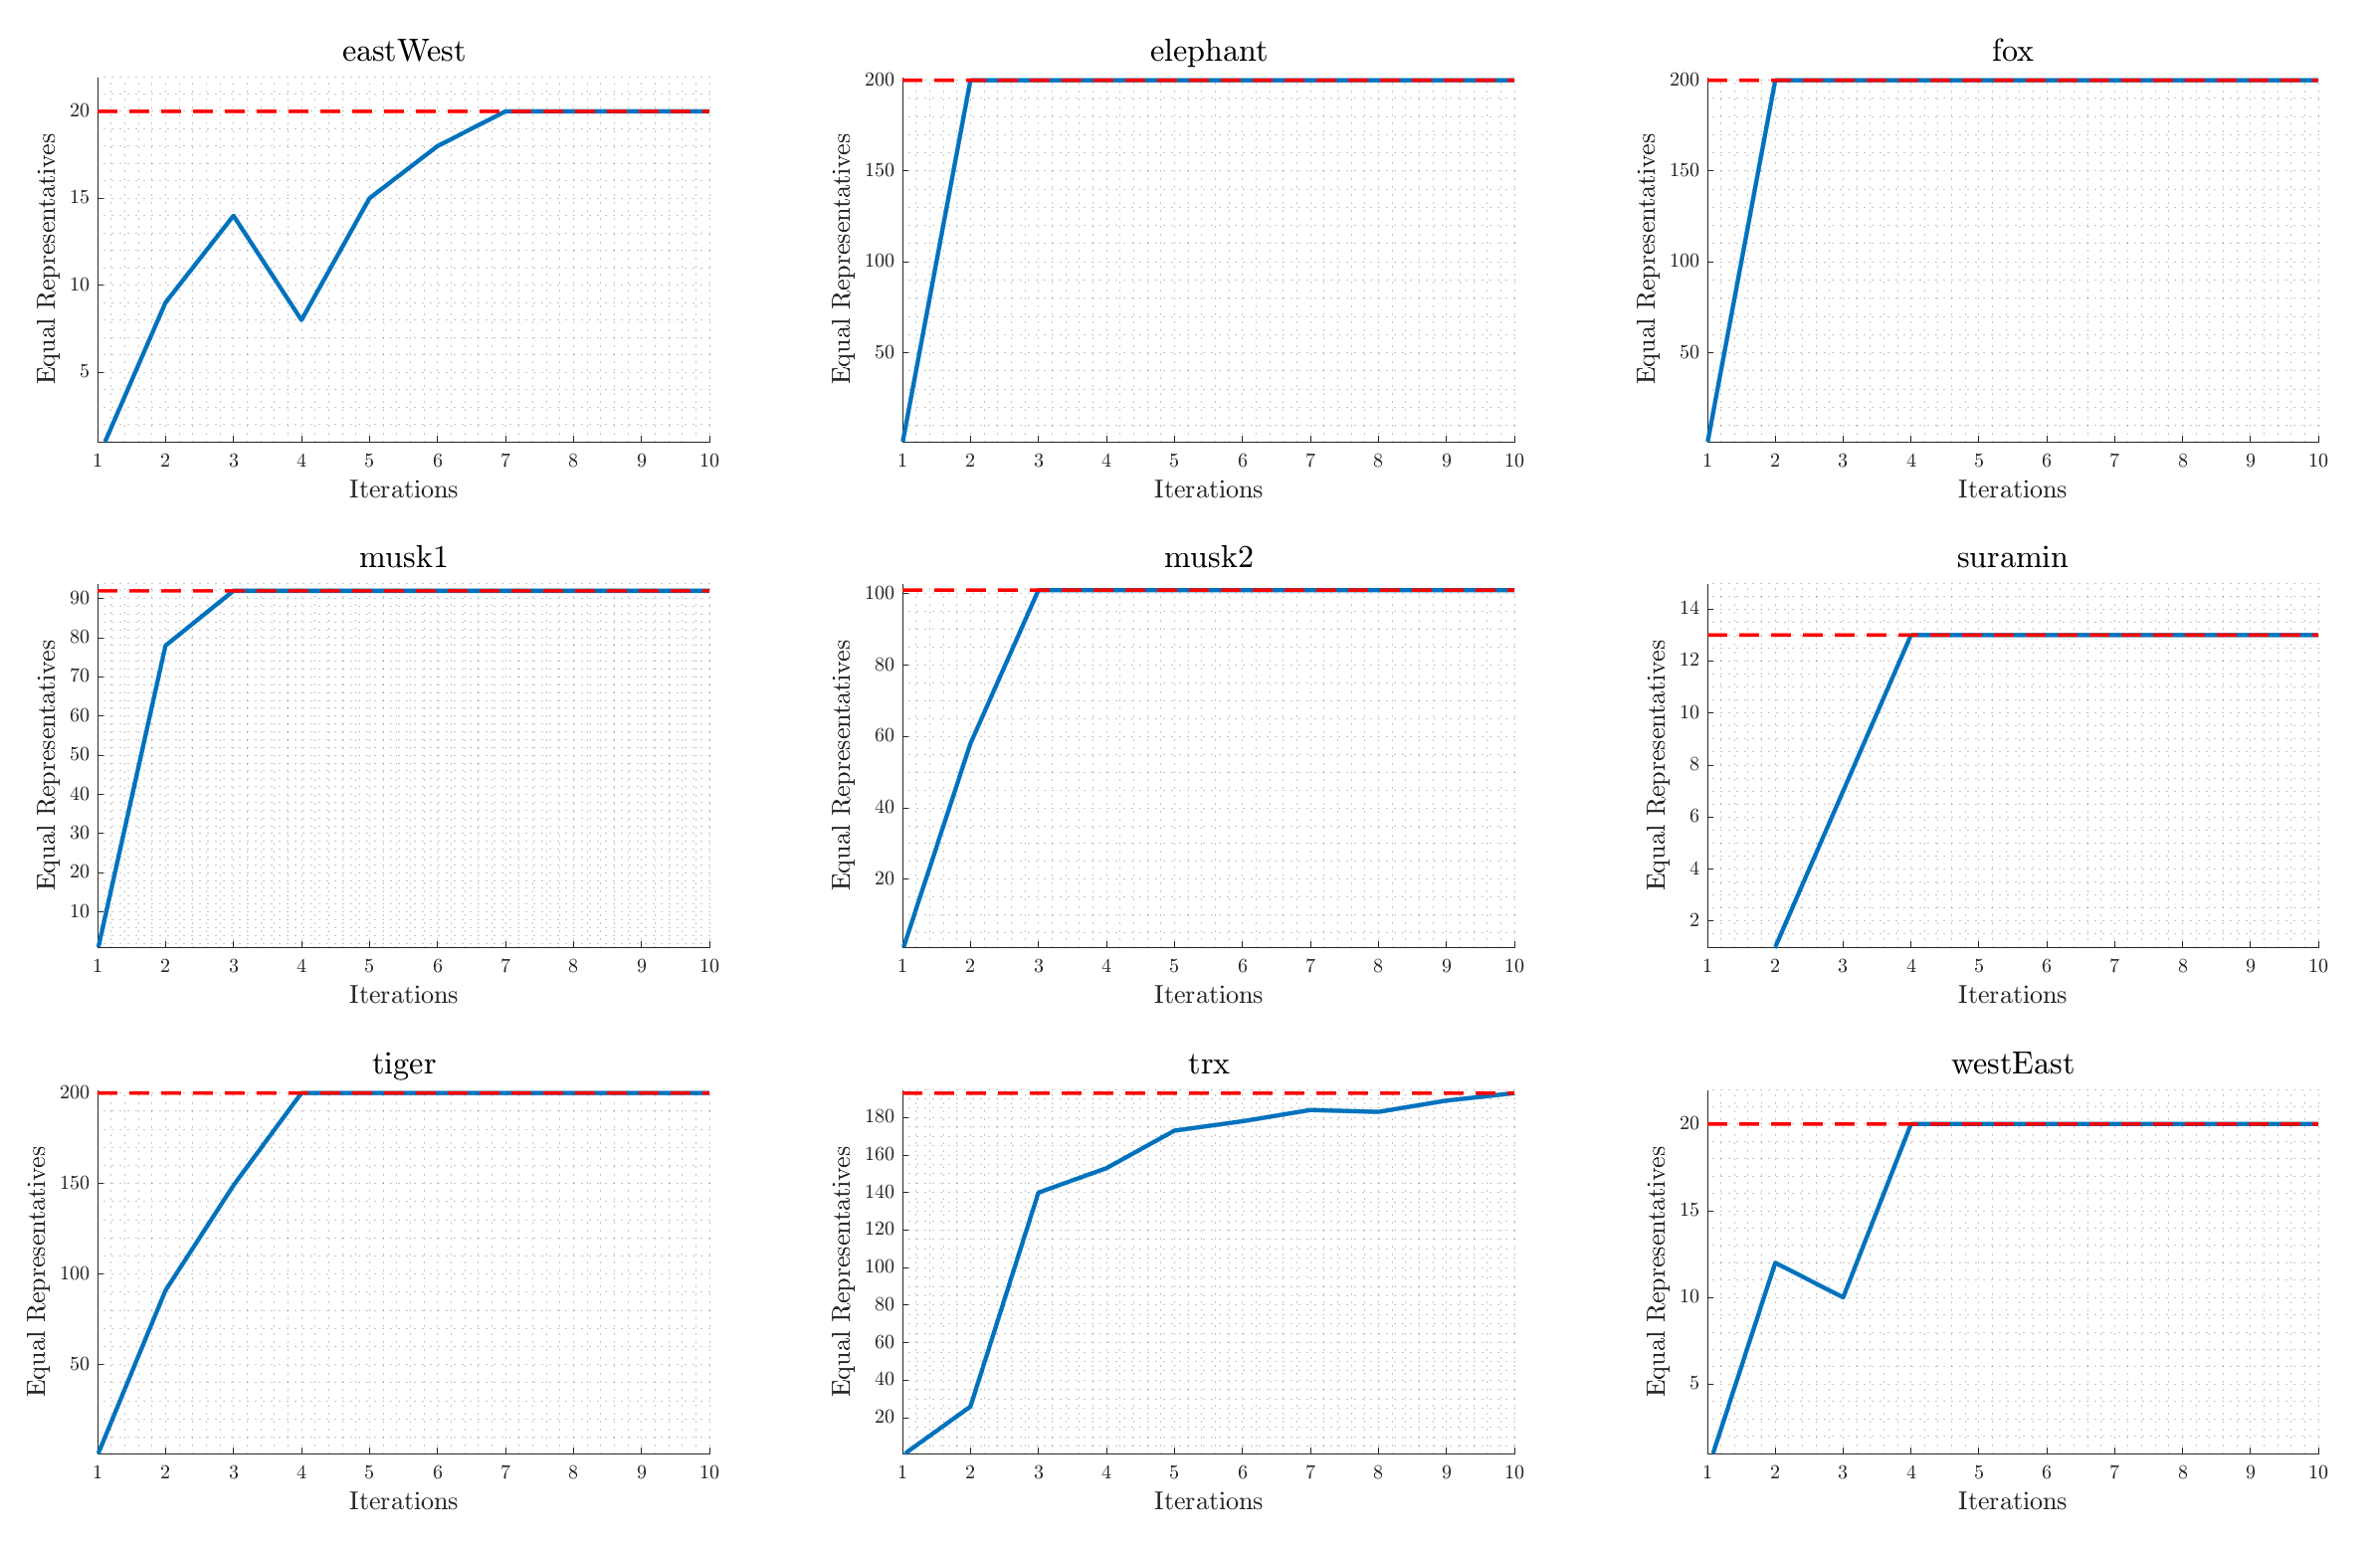
\includegraphics[width=0.94\textwidth]{convergence.png} 
\caption{Bag representative convergence plots on 9 datasets. The blue line shows the number of bag representatives that are equal from one iteration to the next. The red dashed line represents the total number of bags.}
\end{figure}
To evaluate the output vector, $\bm o_I$, of bag $I$ using the kernel, the following equation is used~\citep{Huang2006}, where $\mathcal{B}_I$ are the instances of bag $I$, $\bm X_S$ are the optimal bag representatives, and $\bm Y_S$ are the representative bag labels.
\begin{align}
\bm o_I = \spa{K}(\mathcal{B}_I,\bm X_S)*(\bm\alpha \cdot \bm Y_S) + b
\end{align}

The bias term $b$ is calculated as shown in Equation~\eqref{eqn:bias}, where $\bm{sv}$ is the vector of support vector indices and $n_{sv}$ is the number of support vectors~\citep{Huang2006}.
\begin{align}
\label{eqn:bias}
b = \frac{1}{n_{\bm{sv}}}\sum_{\bm{sv}} Y_{\bm{sv}} - \spa{K}(\bm X_{\bm{sv}},\bm X_{\bm{sv}})*(\bm \alpha_{\bm{sv}}\bm\cdot Y_{\bm{sv}})
\end{align}

Algorithm~\ref{alg:mirsvm} shows the procedure for training the multi-instance representative SVM classifier and obtaining the optimal representatives from each bag.  During training, the representatives, $\bm S$, are first initialized by randomly selecting an instance from each bag. A hyper-plane is then obtained using the representative instances, and new optimal representatives are found with respect to the current hyper-plane, by using the rule given in Equation~\eqref{eq:si}. At each step, the previous values in $\bm S$ are stored in $\bm S_{old}$. The training procedure ends when the bag representatives stop changing from one iteration to the next ($\bm S = \bm S_{old}$). Examples of the convergence of bag-representatives are shown in Figure~\ref{fig:convegence}. During the testing procedure, each bag produces an output vector based on the hyper-plane found in the training procedure. The bag label is then assigned by taking the sign of the output vector's maximum value, following the SMI assumption. 

\begin{figure}
    \centering
    \begin{minipage}{0.5\textwidth}
        \centering
        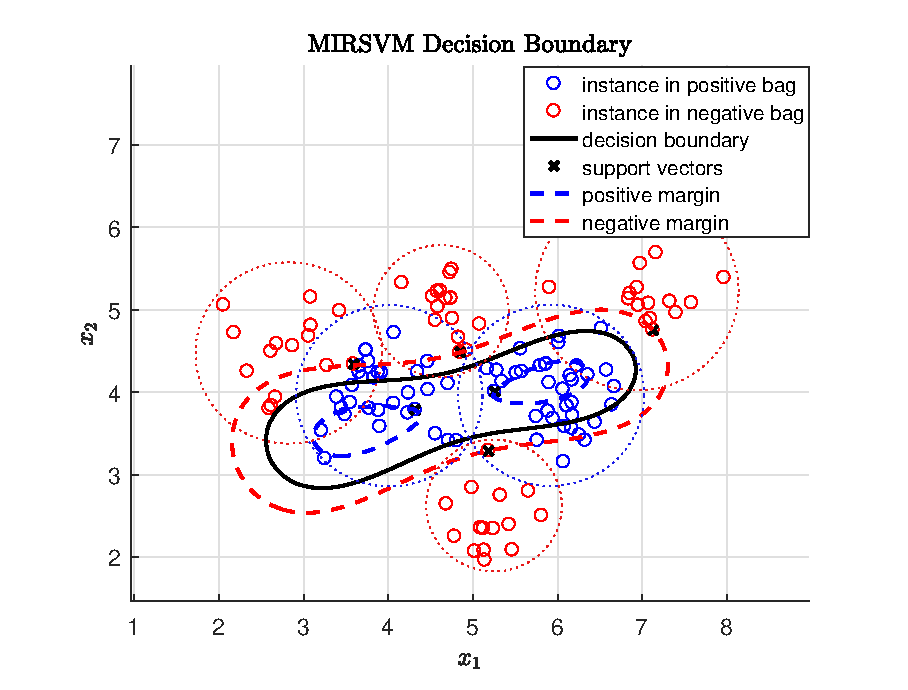
\includegraphics[width=\textwidth]{mirsvm_figure.eps} % first figure itself
    \end{minipage}\hfill
    \begin{minipage}{0.5\textwidth}
        \centering
        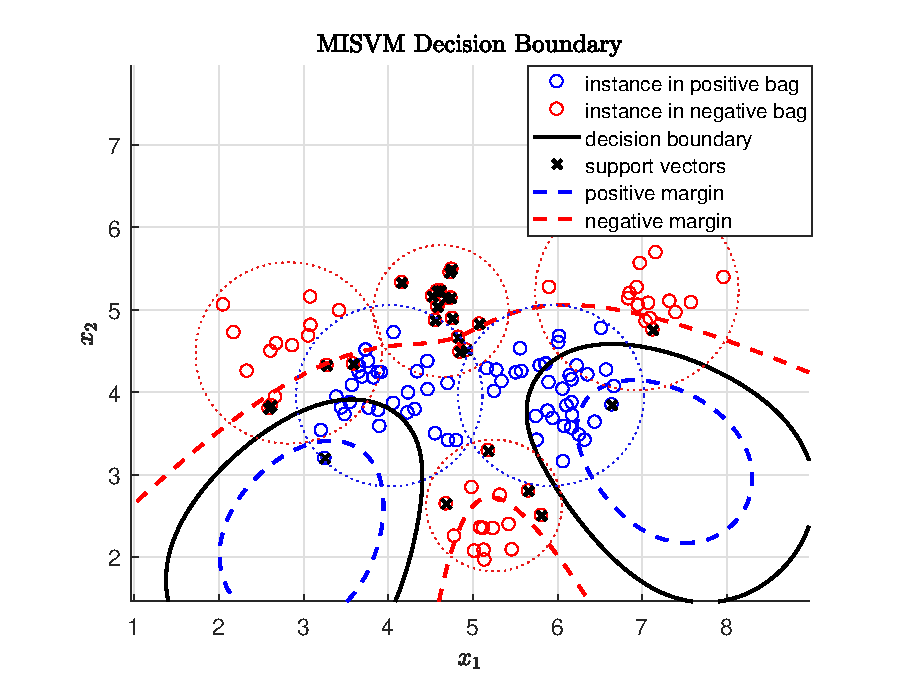
\includegraphics[width=\textwidth]{misvm_figure.eps} % second figure itself
    \end{minipage}
    \caption{Difference between MIRSVM and MISVM on a random $2$-dimensional toy dataset. The instances of this dataset were drawn from the standard normal distribution, with $6$ bags, $4$ of which are negative (red) and $2$ of which are positive (blue), indicated by the red and blue dotted circles. There are a total of $125$ instances, $65$ belonging to the positive bags and $60$ belonging to the negative bags. The decision boundaries (black lines) are shown for each of the algorithms, along with the SVM margin (red and blue dashed lines) and support vectors (black crosses). In this example, both MIRSVM and MISVM were trained using $C = 1000$ and $\sigma = 1.5$. Note the differing number of support vectors produced by the two methods. MIRSVM has $6$, one for each bag, and MISVM has $29$. Also note the smoother representation of the data distribution given by MIRSVM's decision boundary, unlike MISVM whose decision boundary was greatly affected by the larger number of support vectors belonging to the negative class with respect to the only $2$ positive support vectors. }\label{fig:diff}
\end{figure}
\newpage
This formulation is designed to utilize and select representatives from positive and negative bags, unlike MISVM, which only optimizes over representatives from positive bags, while flattening the negative bag instances. MISVM allows multiple representatives to be chosen from negative bags and limits positive bag-representatives to be one, while MIRSVM allows for balanced bag-representative selection, where each bag is allowed one. MISVM also uses a wrapper method to initialize the positive bag-representatives by taking the mean vector of the instances within each positive bag. This is an implicit assumption that the instances within the positive bags are all positive, whereas MIRSVM's initialization procedure selects an instance from all bags at random, ensuring no noise is added by any wrapper techniques during initialization and no assumptions are made about the instances. Due to the constraints on the representatives, MIRSVM produces sparser models while MISVM has the freedom to select as many negative support vectors as it needs and restricts the support vectors chosen from positive bags to be one. Figure~\ref{fig:diff} shows the decision boundaries produced by MIRSVM and MISVM to highlight the differences in their solutions. As Figure~\ref{fig:diff} shows, MISVM produces a larger number of support vectors from the negative bags, which greatly influences the final decision boundary in favor of the negative class.
\newpage
\section{Experiments}\label{sec:experiments}
This section presents the experimental setup and comparison of our contribution, as well as eleven other state-of-the-art methods on $15$ different benchmark datasets. First, the experimental setup is described and the state-of-the-art methods are listed. The results for each metric, as well as the statistical analysis~\citep{ulas2012M2Test}, are then presented and analyzed. Finally, the run-time and meta-ranks of each algorithm are shown, and the overall performance of the algorithms across each metric is discussed. The main aim of the experiments is to compare our contribution to other multi-instance support vector machines, state-of-the-art multi-instance learners, and ensemble methods. 

\subsection{Experimental Setup}
Table~\ref{tab:Dataset} presents a summary of the $15$ datasets used throughout the experiments, where the number of attributes, bags, and total number of instances are shown. The datasets were obtained from the Weka\footnote{http://www.cs.waikato.ac.nz/ml/weka}~\citep{Hall2009} and KEEL\footnote{http://sci2s.ugr.es/keel/datasets.php}~\citep{Alca2011} dataset repositories. 

\begin{table}[t!]
\caption{Datasets used for the experiments in~\ref{subsec:results}}
\small
\label{tab:Dataset}
\begin{tabularx}{\textwidth}{l@{\extracolsep{\fill}}cccccc}
\hline\noalign{\smallskip}
Dataset & Attributes & Positive Bags & Negative Bags & Total & Instances & Average Bag Size\\
\noalign{\smallskip}\hline\noalign{\smallskip}
Suramin & 20 & 7 & 6 & 13 & 2898 &  222.92 \\ 
EastWest & 24 & 10 & 10 & 20 & 213 &  10.65  \\ 
WestEast & 24 & 10 & 10 & 20 & 213 &  10.65  \\ 
Musk1 & 166 & 47 & 45 & 92 & 476 &  5.17  \\ 
Musk2 & 166 & 39 & 62 & 101 & 6728 &  66.61  \\ 
Webmining & 5863 & 21 & 92 & 113 & 3423 &  30.29  \\ 
Mutagenesis-atoms & 10 & 125 & 63 & 188 & 1618 &  8.61  \\ 
Mutagenesis-bonds & 16 & 125 & 63 & 188 & 4081 &  21.71  \\ 
Mutagenesis-chains & 24 & 125 & 63 & 188 & 5424 &  28.85  \\ 
TRX & 8 & 25 & 168 & 193 & 26611 &  137.88 \\ 
Elephant & 230 & 100 & 100 & 200 & 1391 &  6.96 \\ 
Fox & 230 & 100 & 100 & 200 & 1320 &  6.60 \\ 
Tiger & 230 & 100 & 100 & 200 & 1188 &  5.94  \\ 
Component & 200 & 423 & 2707 & 3130 & 36894 &  11.79  \\ 
Function & 200 & 443 & 4799 & 5242 & 55536 &  10.59  \\ 
\noalign{\smallskip}\hline
\end{tabularx}
\end{table}

The experimental environment was designed to test the difference in performance of the proposed method against $11$ state-of-the-art algorithms, contrasting instance-level, bag-level, and ensemble methods. Instance-level methods include MIOptimalBall, MIBoost, MISVM, MIDD, and MIWrapper. Bag-level methods include MISMO, SimpleMI, miGraph, and TLC. The ensemble-based bag-space methods, Bagging and Stacking, were also used. The base algorithms selected for the ensembles Bagging and Stacking were TLC, and TLC and SimpleMI, respectively. These algorithms were chosen because they have shown considerable performance in learning multi-instance models, while also having their frameworks readily available for reproducing their results through MILK, the Multi-Instance Learning Kit\footnote{http://www.cs.waikato.ac.nz/ml/milk}~\citep{Xu2003}, used in conjunction with the Weka framework. Experiments were run on an Intel i7-6700k CPU with 32GB RAM. MIRSVM was implemented in MATLAB while the referenced algorithms are available in the Java implementation of Weka with the exception of miGraph which was made available by Zhou et al.\footnote{http://lamda.nju.edu.cn/code\_miGraph.ashx} and tested in MATLAB.

Experiments were performed using $10$-fold cross validation in order to objectively evaluate the models' performances and tune hyper-parameters. The data is separated fairly into $10$ equally sized sections where, at every iteration of the cross-validation loop, a section is held out as the test set, while the remainder of the data is used for training. These sets are stored and used by each algorithm, ensuring the cross-validation folds are controlled for each algorithm. This procedure ensures the model is not optimistically biased towards the full dataset and the algorithms are evaluated fairly over the same data in each fold. The tuning of the model during cross-validation includes finding the best penalty parameter, $C$, as well as the best shape parameter for the Gaussian radial basis function kernel, $\sigma$. The best hyper-parameters were chosen from the following $6 \times 6$ possible combination runs, shown in Equations~\eqref{eq:paramC} and~\eqref{eq:paramG}, referred to as~\eqref{eq:hyperparam}. 
\begin{subequations}
\label{eq:hyperparam}
\begin{align}
C \in  & \{0.1, 1, 10, 100, 1000, 10000\} \label{eq:paramC}\\
\sigma \in  & \{0.1, 0.5, 1, 2, 5, 10\} \label{eq:paramG}
\end{align}
\end{subequations}

These parameters were also used for the state-of-the-art SVM methods. This was done in order to keep the experimental environment controlled and ensure fair evaluation of the multi-instance SVM algorithms. The parameters for the referenced algorithms used throughout the experiments were those specified by their authors.

\subsection{Results \& Statistical Analysis}\label{subsec:results}
The classification performance was measured using five metrics: Accuracy~\eqref{eq:accuracy}, Precision \eqref{eq:precision}, Recall~\eqref{eq:recall}, Cohen's kappa rate~\eqref{eq:kappa}, and Area under ROC curve (AUC)~\eqref{eq:auc}. The Precision and Recall measures were reported because Accuracy alone can be misleading when classes are imbalanced, as is the case with the \textit{component} and \textit{function} datasets, which respectively have six and ten times as many negative bags than positive. Cohen's Kappa Rate and the AUC measures are used as complementary measures in order to evaluate the algorithms comprehensively~\citep{Bendavid2008}. Cohen's kappa rate, shown in Equation~\eqref{eq:kappa}, evaluates classifier merit according to the class distribution and ranges between -1 (full disagreement), 0 (random classification), and 1 (full agreement). The AUC metric highlights the trade-off between the true positive rate, or recall, and the false positive rate, as shown in Equation~\eqref{eq:auc}. The values of the true positive (TP), true negative (TN), false positive (FP), and false negative samples (FN) were first collected for each of the classifiers, then the metrics were computed using the equations shown in~\eqref{eq:metrics} on the $n^\prime$ bags of the test data, where $n^\prime = TP + FP + TN + FN$. The run times (training and testing times) of each algorithm are also reported to analyze the scalability and speed of each of the algorithms across differently sized datasets. 

The results for the following are shown in Tables~\ref{tab:accResults},~\ref{tab:preResults},~\ref{tab:recResults},~\ref{tab:kappaResults},~\ref{tab:aucResults}, and~\ref{tab:time}.
\begin{subequations}
\label{eq:metrics}
\begin{align}
\text{Accuracy} \tab \tab &\dfrac{TP+TN}{n^\prime} \label{eq:accuracy}\\[10pt]
\text{Precision} \tab \tab &\dfrac{TP}{TP+FP} \label{eq:precision}\\[10pt]
\text{Recall} \tab \tab &\dfrac{TP}{TP+FN} \label{eq:recall}\\[10pt]
\text{Cohen's Kappa Rate} \tab \tab &\dfrac{n^\prime - \dfrac{(TP+FN)*(TP+FP)}{n^\prime}}{1 - \dfrac{(TP+FN)*(TP+FP)}{n^\prime}} \label{eq:kappa}\\[10pt]
\text{Area Under ROC Curve} \tab \tab &\frac{1 + \dfrac{TP}{TP+FN} - \dfrac{FP}{FP+TN}}{2} \label{eq:auc}
\end{align}
\end{subequations}

In order to analyze the performances of the multiple models, non-parametric statistical tests are used to validate the experimental results obtained~\citep{Derrac2011,Garcia20102044}. The Iman-Davenport non-parametric test is run to investigate whether significant differences exist among the performance of the algorithms~\citep{Garcia2008} by ranking them over the datasets used, using the Friedman test. The algorithm ranks for each metric in Equations~\eqref{eq:metrics} are presented in the last row of the results tables, and the lowest (best) rank value is typeset in bold. Table~\ref{tab:metarank} contains the ranks and meta-rank of all methods, which helps determine and visualize the best performing algorithms across all datasets and metrics. 

After the Iman-Davenport test indicates significant differences, the Bonferroni-Dunn post-hoc test~\citep{Dunn1961} is then used to find where they occur between algorithms by assuming the classifiers' performances are different by at least some critical value~\citep{Garcia2009}. Below each result table, a figure highlighting the critical distance (in gray), from the best ranking algorithm to the rest, is shown. The algorithms to the right of the critical distance bar perform statistically significantly worse than the control algorithm, MIRSVM. Figures \ref{fig:BonfDunnacc}, \ref{fig:BonfDunnprec}, \ref{fig:BonfDunnrec}, \ref{fig:BonfDunnkappa}, \ref{fig:BonfDunnauc}, \ref{fig:BonfDunnpmeta} show the results of the Bonferroni-Dunn post-hoc procedure over the metrics in~\eqref{eq:metrics}, as well as the meta-rank results in Table~\ref{tab:metarank}.

The Holm (multiple) and Wilcoxon (pairwise) rank-sum post-hoc tests~\citep{Gibbons2011,Holander1999} were then run for each of the metrics to compute multiple and pairwise comparisons between the proposed algorithm and the state-of-the-art methods, investigating whether statistical differences exist among the algorithms' results. Tables~\ref{tab:statacc},~\ref{tab:statprec},~\ref{tab:statrec},~\ref{tab:statkappa}, and~\ref{tab:statauc} show the $p$-values for the Holm test for $\alpha = 0.05$, and the rank-sums and adjusted $p$-values for the Wilcoxon test.
\newpage
\subsection{Accuracy}
\begin{table}[t!]
\caption{Accuracy}\label{tab:accResults}
\resizebox{0.95\textwidth}{!}{\begin{tabular}{l@{\extracolsep{\fill}}ccccccccccccc}
\noalign{\smallskip}\hline\noalign{\smallskip}
Datasets &MIRSVM & miGraph & MIBoost &MIOptimalBall &MIDD &MIWrapper &MISMO &MISVM &SimpleMI &TLC &Bagging &Stacking \\
\noalign{\smallskip}\hline\noalign{\smallskip}
suramin &0.8000 &\textbf{0.8462} &0.5000 &0.7250 &0.4250 &0.5000 &0.7250 &0.5000 &0.5000 &0.6000 &0.6650 &0.4615 &  \\
eastWest &\textbf{0.8000} &0.7000 &0.5000 &0.7250 &0.6125 &0.5000 &0.7125 &0.5625 &0.5000 &0.6000 &0.6000 &0.4500 &  \\
westEast &0.7500 &0.7500 &0.5000 &0.3750 &0.4500 &0.5000 &0.7375 &0.4125 &0.5000 &0.5625 &\textbf{0.9649} &0.6375 &  \\
musk1 &\textbf{0.9022} &0.8152 &0.5109 &0.7717 &0.8804 &0.5109 &0.7826 &0.7609 &0.5109 &0.8587 &0.8142 &0.8587 &  \\
musk2 &0.8218 &0.7426 &0.6139 &0.7723 &0.7228 &0.6139 &0.7030 &0.7129 &0.6139 &0.6238 &\textbf{0.8756} &0.6733 &  \\
webmining &0.8500 &0.8142 &0.8142 &0.7699 &0.8142 &0.8142 &0.8407 &0.6903 &0.8142 &0.8142 &\textbf{0.9358} &0.8053 &  \\
trx &0.8860 &0.8964 &0.8705 &\textbf{0.9016} &0.8808 &0.8705 &0.8705 &0.8705 &0.8705 &0.8756 &0.6450 &0.8860 &  \\
mutagenesis-atoms &0.7714 &0.7606 &0.6649 &0.6436 &0.7074 &0.6649 &0.6915 &0.6649 &0.6649 &\textbf{0.7766} &\textbf{0.7766} &0.7606 &  \\
mutagenesis-bonds &0.8252 &0.7872 &0.6649 &0.6915 &0.7713 &0.6649 &0.7979 &0.6649 &0.6649 &0.8351 &0.8351 &\textbf{0.8564} &  \\
mutagenesis-chains &\textbf{0.8411} &0.7926 &0.6649 &0.6702 &0.7766 &0.6649 &0.8351 &0.6649 &0.6649 &0.8404 &0.8404 &0.8351 &  \\
tiger &0.7750 &0.7950 &0.5000 &0.5000 &0.7100 &0.5000 &0.7200 &0.7550 &0.5000 &0.6650 &\textbf{0.8000} &0.7250 &  \\
elephant &\textbf{0.8300} &\textbf{0.8300} &0.5000 &0.5000 &0.7900 &0.5000 &0.8100 &0.8000 &0.5000 &0.8000 &0.5625 &0.8250 &  \\
fox &0.6550 &0.6300 &0.5000 &0.5000 &0.5800 &0.5000 &0.5250 &0.4750 &0.5000 &0.6450 &\textbf{0.8587} &0.6500 &  \\
component &\textbf{0.9366} &0.9153 &0.8649 &0.8696 &0.8780 &0.8649 &0.8968 &0.8703 &0.8649 &0.9358 &0.6000 &0.9355 &  \\
function &0.9523 &0.9405 &0.9155 &0.9138 &0.9193 &0.9155 &0.9376 &0.9195 &0.9155 &\textbf{0.9649} &0.6238 &0.9647 &  \\
\noalign{\smallskip}\hline\noalign{\smallskip}
Average &\textbf{0.8264} &0.8010 &0.6390 &0.6886 &0.7279 &0.6390 &0.7724 &0.6883 &0.6390 &0.7598 &0.7598 &0.7550 &  \\
Rank &\textbf{2.2000} &3.8667 &9.6000 &7.8667 &6.5667 &9.6000 &5.3333 &8.5667 &9.6000 &4.7000 &4.8667 &5.2333 &  \\
\noalign{\smallskip}\hline
\end{tabular}}
\centering
\resizebox{0.95\textwidth}{!}{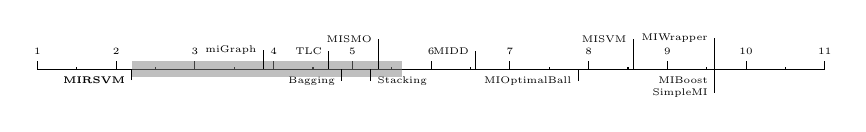
\begin{tikzpicture}
\draw (1,0) -- (11,0);
\foreach \x in {1,2,3,4,5,6,7,8,9,10,11} {
\draw (\x, 0) -- ++(0,.1) node [above,scale=0.7] {\tiny \x};
\ifthenelse{\x < 11}{\draw (\x+.5, 0) -- ++(0,.03);}{}
}

\coordinate (c0) at (2.2,0);
\coordinate (c1) at (3.8667,0);
\coordinate (c2) at (9.6,0);
\coordinate (c3) at (7.8667,0);
\coordinate (c4) at (6.5667,0);
\coordinate (c5) at (9.6,0);
\coordinate (c6) at (5.3333,0);
\coordinate (c7) at (8.5667,0);
\coordinate (c8) at (9.6,0);
\coordinate (c9) at (4.7,0);
\coordinate (c10) at (4.8667,0);
\coordinate (c11) at (5.2333,0);

\node (l0) at (c0) [below left=.01cm and 0cm, align=right,scale=0.7] {\tiny \textbf{MIRSVM}};
\node (l1) at (c1) [above left=.1cm and 0cm, align=right,scale=0.7] {\tiny miGraph};
\node (l2) at (c2) [below left=.01cm and 0cm, align=right,scale=0.7] {\tiny MIBoost};
\node (l3) at (c3) [below left=.01cm and 0cm, align=right,scale=0.7] {\tiny MIOptimalBall};
\node (l4) at (c4) [above left=.1cm and 0cm, align=right,scale=0.7] {\tiny MIDD};
\node (l5) at (c5) [above left=.25cm and 0cm, align=right,scale=0.7] {\tiny MIWrapper};
\node (l6) at (c6) [above left=.25cm and 0cm, align=right,scale=0.7] {\tiny MISMO};
\node (l7) at (c7) [above left=.25cm and 0cm, align=right,scale=0.7] {\tiny MISVM};
\node (l8) at (c8) [below left=.16cm and 0cm, align=right,scale=0.7] {\tiny SimpleMI};
\node (l9) at (c9) [above left=.1cm and 0cm, align=right,scale=0.7] {\tiny TLC};
\node (l10) at (c10) [below left=.01cm and 0cm, align=right,scale=0.7] {\tiny Bagging};
\node (l11) at (c11) [below right=.01cm and 0cm, align=left,scale=0.7] {\tiny Stacking};

\fill[fill=gray,fill opacity=0.5] (2.2,-0.1) rectangle (5.635,0.1);

\foreach \x in {0,1,2,3,4,5,6,7,8,9,10,11} {
\draw (l\x) -| (c\x);
};
\end{tikzpicture}}\vspace{-0.6em}
\captionof{figure}{Bonferroni-Dunn test for Accuracy}\label{fig:BonfDunnacc}\vspace{-0.5em}
\captionof{table}{Holm and Wilcoxon tests for Accuracy}\label{tab:statacc}
\scriptsize
\resizebox{0.95\textwidth}{!}{\begin{tabular}{lccccccccccc}
\noalign{\smallskip}\hline\noalign{\smallskip}
MIRSVM vs. &miGraph &MIBoost &MIOptimalBall &MIDD &MIWrapper &MISMO &MISVM &SimpleMI &TLC &Bagging &Stacking \\
\noalign{\smallskip}\hline\noalign{\smallskip}
Holm $p$-value &0.0500 &0.0045 &0.0071 &0.0083 &0.0050 &0.0100 &0.0063 &0.0056 &0.0250 &0.0167 &0.0125 \\\noalign{\smallskip}\hline\noalign{\smallskip}
Wilcoxon $p$-value &0.0279 &0.0001 &0.0001 &0.0001 &0.0001 &0.0001 &0.0001 &0.0001 &0.0067 & 0.3028 &0.0103 \\
Wilcoxon R$^+$ &98.500 &120.00 &119.00 &120.00 &120.00 &120.00 &120.00 &120.00 &106.00 &79.000 &104.00 \\
Wilcoxon R$^-$ &21.500 & 0.0000 &1.0000 & 0.0000 &0.0000 &0.0000 &0.0000 &0.0000 &14.000 &41.000 &16.000 \\
\noalign{\smallskip}\hline\noalign{\smallskip}
\end{tabular}}
\end{table}
Table~\ref{tab:accResults} shows the accuracy results of the $11$ algorithms over $15$ multi-instance datasets, along with their average and rank. The results indicate that the bag-based and ensemble learners perform better than the instance-based and wrapper methods. Specifically, MIRSVM achieves the best accuracy over $5$ of the $15$ datasets with a competitive average against the miGraph, Bagging, Stacking, and TLC algorithms. Note that MIRSVM performs better than MISVM for all datasets, indicating that using representatives from each bag and limiting the number of support-vectors per negative bag improves the classification performance. The instance-level classifiers and wrapper methods, such as MIBoost, MIWrapper, and SimpleMI perform the worst. This behavior emphasizes the importance of not making prior assumptions about the positive bags' distributions. 

Figure~\ref{fig:BonfDunnacc} and Table~\ref{tab:statacc} show the results for the statistical analysis on the accuracy results. The algorithms with ranking higher than $5.63$ (MIRSVM rank + Bonferroni-Dunn critical value), to the right of the grey bar in Figure~\ref{fig:BonfDunnacc}, perform statistically worse than MIRSVM. Table~\ref{tab:statacc} shows the $p$-values of the Holm and Wilcoxon tests and their results complement one another. Holm's procedure rejects those hypotheses having a $p$-value $\leq 0.01$, thus indicating that MIRSVM performs significantly better than all methods except miGraph, Bagging, Stacking, and TLC. The Wilcoxon $p$-values show significant differences exist among all algorithms except miGraph, Bagging, and Stacking. They also show that MIRSVM has significantly better accuracy than MIBoost, MIOptimalBall, MIDD, MIWrapper, MISMO, MISVM, and SimpleMI, each having respectively small $p$-values, highlighting MIRSVM's superior classification accuracy. 

\begin{table}[H]
\caption{Precision}\label{tab:preResults}
\resizebox{0.95\textwidth}{!}{\begin{tabular}{l@{\extracolsep{\fill}}ccccccccccccc}
\noalign{\smallskip}\hline\noalign{\smallskip}
Datasets &MIRSVM & miGraph & MIBoost &MIOptimalBall &MIDD &MIWrapper &MISMO &MISVM &SimpleMI &TLC &Bagging &Stacking \\
\noalign{\smallskip}\hline\noalign{\smallskip}
suramin &0.7778 &0.7778 &\textbf{1.0000} &\textbf{1.0000} &0.2857 &\textbf{1.0000} &\textbf{1.0000} &0.5000 &\textbf{1.0000} &0.6429 &0.6514 &0.4000 &  \\
eastWest &0.7143 &0.7000 &0.5000 &0.8750 &0.5882 &0.5000 &0.7429 &\textbf{1.0000} &0.5000 &0.6053 &0.6053 &0.4444 &  \\
westEast &0.7272 &0.7273 &0.5000 &0.2727 &0.4600 &0.5000 &0.6939 &0.3600 &0.5000 &0.5581 &\textbf{0.9729} &0.6038 &  \\
musk1 &0.8519 &0.7778 &\textbf{1.0000} &0.9286 &0.9048 &\textbf{1.0000} &0.8049 &0.8108 &\textbf{1.0000} &0.8478 &0.8817 &0.8478 &  \\
musk2 &0.7059 &0.7826 &0.6139 &0.7826 &0.7576 &0.6139 &0.7424 &0.7538 &0.6139 &0.7400 &\textbf{0.9138} &0.7164 &  \\
webmining &0.7500 &\textbf{1.0000} &0.8142 &0.8173 &0.8142 &0.8142 &0.8936 &\textbf{1.0000} &0.8142 &0.8817 &0.9462 &0.8500 &  \\
trx &\textbf{1.0000} &0.8571 &0.8705 &0.9306 &0.9191 &0.8705 &0.8705 &0.8705 &0.8705 &0.9138 &0.6747 &0.9011 &  \\
mutagenesis-atoms &0.7872 &0.7985 &\textbf{1.0000} &0.4630 &0.6111 &\textbf{1.0000} &0.5439 &\textbf{1.0000} &\textbf{1.0000} &0.7059 &0.7059 &0.6667 &  \\
mutagenesis-bonds &0.8468 &0.8195 &\textbf{1.0000} &0.5385 &0.7500 &\textbf{1.0000} &0.6812 &\textbf{1.0000} &\textbf{1.0000} &0.7857 &0.7857 &0.8333 &  \\
mutagenesis-chains &0.8571 &0.8116 &\textbf{1.0000} &0.5091 &0.7059 &\textbf{1.0000} &0.7759 &\textbf{1.0000} &\textbf{1.0000} &0.7705 &0.7705 &0.7581 &  \\
tiger &0.7365 &0.7323 &0.5000 &0.5000 &0.6944 &0.5000 &0.7444 &0.7802 &0.5000 &0.6514 &\textbf{0.8000} &0.7320 &  \\
elephant &0.8576 &\textbf{0.8750} &0.5000 &0.5000 &0.7959 &0.5000 &0.8444 &0.7679 &0.5000 &0.8000 &0.5581 &0.8283 &  \\
fox &0.6040 &0.6275 &0.5000 &0.5000 &0.5833 &0.5000 &0.5287 &0.4854 &0.5000 &0.6747 &\textbf{0.8478} &0.6705 &  \\
component &\textbf{0.9866} &0.7782 &0.8649 &0.8778 &0.8902 &0.8649 &0.8958 &0.8696 &0.8649 &0.9462 &0.6429 &0.9449 &  \\
function &0.8459 &0.6775 &0.9155 &0.9202 &0.9317 &0.9155 &0.9376 &0.9197 &0.9155 &\textbf{0.9729} &0.7400 &0.9726 &  \\
\noalign{\smallskip}\hline\noalign{\smallskip}
Average &0.8033 &0.7828 &0.7719 &0.6944 &0.7128 &0.7719 &0.7800 &\textbf{0.8079} &0.7719 &0.7665 &0.7665 &0.7447 &  \\
Rank &\textbf{5.3333} &6.1333 &7.1000 &7.3333 &7.3667 &7.1000 &5.8667 &5.8667 &7.1000 &5.9000 &6.3333 &6.5667 &  \\
\noalign{\smallskip}\hline
\end{tabular}}
\centering
\resizebox{0.95\textwidth}{!}{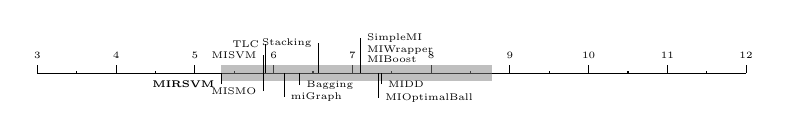
\begin{tikzpicture}
\draw (3,0) -- (12,0);
\foreach \x in {3,4,5,6,7,8,9,10,11,12} {
\draw (\x, 0) -- ++(0,.1) node [above,scale=0.7] {\tiny \x};
\ifthenelse{\x < 12}{\draw (\x+.5, 0) -- ++(0,.03);}{}
}

\coordinate (c0) at (5.3333,0);
\coordinate (c1) at (6.1333,0);
\coordinate (c2) at (7.1,0);
\coordinate (c3) at (7.3333,0);
\coordinate (c4) at (7.3667,0);
\coordinate (c5) at (7.1,0);
\coordinate (c6) at (5.8667,0);
\coordinate (c7) at (5.8667,0);
\coordinate (c8) at (7.1,0);
\coordinate (c9) at (5.9,0);
\coordinate (c10) at (6.3333,0);
\coordinate (c11) at (6.5667,0);

\node (l0) at (c0) [below left=.01cm and 0cm, align=right,scale=0.7] {\tiny \textbf{MIRSVM}};
\node (l1) at (c1) [below right=.16cm and 0cm, align=left,scale=0.7] {\tiny miGraph};
\node (l2) at (c2) [above right=.05cm and 0cm, align=left,scale=0.7] {\tiny MIBoost};
\node (l3) at (c3) [below right=.17cm and 0cm, align=left,scale=0.7] {\tiny MIOptimalBall};
\node (l4) at (c4) [below right=.01cm and 0cm, align=left,scale=0.7] {\tiny MIDD};
\node (l5) at (c5) [above right=.15cm and 0cm, align=left,scale=0.7] {\tiny MIWrapper};
\node (l6) at (c6) [below left=.1cm and 0cm, align=right,scale=0.7] {\tiny MISMO};
\node (l7) at (c7) [above left=.1cm and 0cm, align=right,scale=0.7] {\tiny MISVM};
\node (l8) at (c8) [above right=.3cm and 0cm, align=left,scale=0.7] {\tiny SimpleMI};
\node (l9) at (c9) [above left=.24cm and 0cm, align=right,scale=0.7] {\tiny TLC};
\node (l10) at (c10) [below right=.01cm and 0cm, align=left,scale=0.7] {\tiny Bagging};
\node (l11) at (c11) [above left=.24cm and 0cm, align=right,scale=0.7] {\tiny Stacking};

\fill[fill=gray,fill opacity=0.5] (5.3333,-0.1) rectangle (8.7683,0.1);

\foreach \x in {0,1,2,3,4,5,6,7,8,9,10,11} {
\draw (l\x) -| (c\x);};
\end{tikzpicture}}\vspace{-1.1em}
\captionof{figure}{Bonferroni-Dunn test for Precision}\label{fig:BonfDunnprec}\vspace{-0.5em}
\captionof{table}{Holm and Wilcoxon tests for Precision}\label{tab:statprec}
\scriptsize
\resizebox{0.95\textwidth}{!}{\begin{tabular}{lccccccccccc}
\noalign{\smallskip}\hline\noalign{\smallskip}
MIRSVM vs. &miGraph &MIBoost &MIOptimalBall &MIDD &MIWrapper &MISMO &MISVM &SimpleMI &TLC &Bagging &Stacking \\
\noalign{\smallskip}\hline\noalign{\smallskip}
Holm $p$-value &0.0125 &0.0056 &0.0050 &0.0045 &0.0063 &0.0250 &0.0500 &0.0071 &0.0167 &0.0100 &0.0083 \\\noalign{\smallskip}\hline\noalign{\smallskip}
Wilcoxon $p$-value & 0.4212 & 0.5614 &0.0946 &0.0256 & 0.5614 & 0.4212 & 0.8039 & 0.5614 &0.1354 & 0.4543 &0.1354 \\
Wilcoxon R$^+$ &75.000 &71.000 &90.000 &99.000 &71.000 &75.000 &55.000 &71.000 &87.000 &74.000 &87.000 \\
Wilcoxon R$^-$ &45.000 &49.000 &30.000 &21.000 &49.000 &45.000 &65.000 &49.000 &33.000 &46.000 &33.000 \\
\noalign{\smallskip}\hline\noalign{\smallskip}
\end{tabular}}
\captionof{table}{Recall}\label{tab:recResults}
\resizebox{0.95\textwidth}{!}{\begin{tabular}{l@{\extracolsep{\fill}}ccccccccccccc}
\noalign{\smallskip}\hline\noalign{\smallskip}
Datasets &MIRSVM & miGraph & MIBoost &MIOptimalBall &MIDD &MIWrapper &MISMO &MISVM &SimpleMI &TLC &Bagging &Stacking \\
\noalign{\smallskip}\hline\noalign{\smallskip}
suramin &\textbf{1.0000} &\textbf{1.0000} &0.0000 &0.4500 &0.1000 &0.0000 &0.4500 &0.5000 &0.0000 &0.4500 &0.7100 &0.3333 &  \\
eastWest &\textbf{1.0000} &0.7000 &0.7000 &0.5250 &0.7500 &0.7000 &0.6500 &0.1250 &\textbf{1.0000} &0.5750 &0.5750 &0.4000 &  \\
westEast &0.8000 &0.8000 &0.9000 &0.1500 &0.5750 &0.9000 &0.8500 &0.2250 &\textbf{1.0000} &0.6000 &0.9892 &0.8000 &  \\
musk1 &\textbf{0.9787} &0.8936 &0.0000 &0.5778 &0.8444 &0.0000 &0.7333 &0.6667 &0.0000 &0.8667 &0.8913 &0.8667 &  \\
musk2 &0.9231 &0.4615 &\textbf{1.0000} &0.8710 &0.8065 &\textbf{1.0000} &0.7903 &0.7903 &\textbf{1.0000} &0.5968 &0.9464 &0.7742 &  \\
webmining &0.2857 &0.0000 &\textbf{1.0000} &0.9239 &\textbf{1.0000} &\textbf{1.0000} &0.9130 &0.6196 &\textbf{1.0000} &0.8913 &0.9815 &0.9239 &  \\
trx &0.4833 &0.2400 &\textbf{1.0000} &0.9583 &0.9464 &\textbf{1.0000} &\textbf{1.0000} &\textbf{1.0000} &\textbf{1.0000} &0.9464 &0.5600 &0.9762 &  \\
mutagenesis-atoms &\textbf{0.8880} &0.8560 &0.0000 &0.3968 &0.3492 &0.0000 &0.4921 &0.0000 &0.0000 &0.5714 &0.5714 &0.5714 &  \\
mutagenesis-bonds &\textbf{0.8960} &0.8720 &0.0000 &0.5556 &0.4762 &0.0000 &0.7460 &0.0000 &0.0000 &0.6984 &0.6984 &0.7143 &  \\
mutagenesis-chains &\textbf{0.9120} &0.8960 &0.0000 &0.4444 &0.5714 &0.0000 &0.7143 &0.0000 &0.0000 &0.7460 &0.7460 &0.7460 &  \\
tiger &0.8700 &0.9300 &0.5000 &\textbf{1.0000} &0.7500 &0.5000 &0.6700 &0.7100 &\textbf{1.0000} &0.7100 &0.8000 &0.7100 &  \\
elephant &0.9100 &0.7700 &0.6000 &\textbf{1.0000} &0.7800 &0.6000 &0.7600 &0.8600 &\textbf{1.0000} &0.8000 &0.6000 &0.8200 &  \\
fox &0.9000 &0.6400 &0.7000 &\textbf{1.0000} &0.5600 &0.7000 &0.4600 &0.8300 &\textbf{1.0000} &0.5600 &0.8667 &0.5900 &  \\
component &0.5839 &0.5225 &\textbf{1.0000} &0.9867 &0.9797 &\textbf{1.0000} &0.9967 &\textbf{1.0000} &\textbf{1.0000} &0.9815 &0.4500 &0.9826 &  \\
function &0.5327 &0.5643 &\textbf{1.0000} &0.9919 &0.9840 &\textbf{1.0000} &0.9983 &0.9994 &\textbf{1.0000} &0.9892 &0.5968 &0.9894 &  \\
\noalign{\smallskip}\hline\noalign{\smallskip}
Average &\textbf{0.7976} &0.6764 &0.5600 &0.7221 &0.6982 &0.5600 &0.7483 &0.5551 &0.6667 &0.7322 &0.7322 &0.7465 &  \\
Rank &4.8667 &6.5667 &6.8667 &6.3333 &7.3667 &6.8667 &6.7000 &7.4333 &\textbf{4.8333} &7.3667 &6.0667 &6.7333 &  \\
\noalign{\smallskip}\hline
\end{tabular}}
\resizebox{0.95\textwidth}{!}{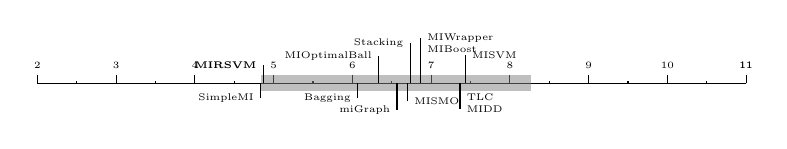
\begin{tikzpicture}
\draw (2,0) -- (11,0);
\foreach \x in {2,3,4,5,6,7,8,9,10,11,11} {
\draw (\x, 0) -- ++(0,.1) node [above,scale=0.7] {\tiny \x};
\ifthenelse{\x < 11}{\draw (\x+.5, 0) -- ++(0,.03);}{}
}

\coordinate (c0) at (4.8667,0);
\coordinate (c1) at (6.5667,0);
\coordinate (c2) at (6.8667,0);
\coordinate (c3) at (6.3333,0);
\coordinate (c4) at (7.3667,0);
\coordinate (c5) at (6.8667,0);
\coordinate (c6) at (6.7,0);
\coordinate (c7) at (7.4333,0);
\coordinate (c8) at (4.8333,0);
\coordinate (c9) at (7.3667,0);
\coordinate (c10) at (6.0667,0);
\coordinate (c11) at (6.7333,0);

\node (l0) at (c0) [above left=.1cm and 0cm, align=right,scale=0.7] {\tiny \textbf{MIRSVM}};
\node (l1) at (c1) [below left=.2cm and 0cm, align=right,scale=0.7] {\tiny miGraph};
\node (l2) at (c2) [above right=.3cm and 0cm, align=left,scale=0.7] {\tiny MIBoost};
\node (l3) at (c3) [above left=.2cm and 0cm, align=right,scale=0.7] {\tiny MIOptimalBall};
\node (l4) at (c4) [below right=.2cm and 0cm, align=left,scale=0.7] {\tiny MIDD};
\node (l5) at (c5) [above right=.43cm and 0cm, align=left,scale=0.7] {\tiny MIWrapper};
\node (l6) at (c6) [below right=.1cm and 0cm, align=left,scale=0.7] {\tiny MISMO};
\node (l7) at (c7) [above right=.23cm and 0cm, align=left,scale=0.7] {\tiny MISVM};
\node (l8) at (c8) [below left=.05cm and 0cm, align=right,scale=0.7] {\tiny SimpleMI};
\node (l9) at (c9) [below right=.05cm and 0cm, align=left,scale=0.7] {\tiny TLC};
\node (l10) at (c10) [below left=.05cm and 0cm, align=right,scale=0.7] {\tiny Bagging};
\node (l11) at (c11) [above left=.37cm and 0cm, align=right,scale=0.7] {\tiny Stacking};

\fill[fill=gray,fill opacity=0.5] (4.8333,-0.1) rectangle (8.2683,0.1);

\foreach \x in {0,1,2,3,4,5,6,7,8,9,10,11} {
\draw (l\x) -| (c\x);};
\end{tikzpicture}}\vspace{-1.1em}
\captionof{figure}{Bonferroni-Dunn test for Recall}\label{fig:BonfDunnrec}\vspace{-0.5em}
\captionof{table}{Holm and Wilcoxon tests for Recall}\label{tab:statrec}
\scriptsize
\resizebox{0.95\textwidth}{!}{\begin{tabular}{lccccccccccc}
\noalign{\smallskip}\hline\noalign{\smallskip}
MIRSVM vs. &miGraph &MIBoost &MIOptimalBall &MIDD &MIWrapper &MISMO &MISVM &SimpleMI &TLC &Bagging &Stacking \\
\noalign{\smallskip}\hline\noalign{\smallskip}
Holm $p$-value &0.0125 &0.0063 &0.0167 &0.0050 &0.0071 &0.0100 &0.0045 &0.0500 &0.0056 &0.0250 &0.0083 \\\noalign{\smallskip}\hline\noalign{\smallskip}
Wilcoxon $p$-value &0.0060 & 0.2077 & 0.5614 & 0.4543 & 0.2077 & 0.6387 &0.1070 & 0.6603 & 0.5995 &0.1354 & 0.5721 \\
Wilcoxon R$^+$ &106.50 &83.000 &71.000 &74.000 &83.000 &69.000 &89.000 &60.000 &70.000 &87.000 &62.000 \\
Wilcoxon R$^-$ &13.500 &37.000 &49.000 &46.000 &37.000 &51.000 &31.000 &45.000 &50.000 &33.000 &43.000 \\
\noalign{\smallskip}\hline\noalign{\smallskip}
\end{tabular}}
\end{table}

\subsection{Precision \& Recall}
Precision and recall are conflicting metrics that must be evaluated together in order to observe their behavior simultaneously, since they are both used to measure relevance. Tables~\ref{tab:preResults} and~\ref{tab:recResults} show the precision and recall results obtained by each algorithm. The precision and recall results for MIWrapper and SimpleMI indicate that they are unstable classifiers, exhibiting extreme variance in behavior, making them unsuitable for real-world applications. It is also interesting to analyze the performance on the mutagenesis datasets which have a larger number of positive bags than negative, where MISVM, MIBoost, MIWrapper, and SimpleMI predict all bags as negative. Additionally, while MISMO obtains unbiased results on these datasets, MIRSVM significantly outperforms it over both precision and recall, achieving a better trade-off.  

Figure~\ref{fig:BonfDunnprec} and~\ref{fig:BonfDunnrec} show that there are no statistically significant differences between the precision and recall results obtained by all algorithms. It is worth noting that MIRSVM outperforms both ensemble methods according to recall, despite them exhibiting relatively good accuracy and precision. This indicates that they are strongly conservative towards predicting positive bags. The Holm test indicates significant differences exist between MIRSVM and all algorithms except miGraph, MISMO, MISVM, and TLC for precision, and all the above along with SimpleMI, MIOptimalBall, and Bagging for recall. The Wilcoxon $p$-values do not reflect significant differences for precision, but they do for recall. The tests' results are severely biased due to the extreme unbalanced behavior of the classifiers, whereas MIRSVM demonstrates proper balance of the precision-recall trade-off.

\subsection{Cohen's Kappa Rate}
\begin{table}[b!]
\caption{Cohen's Kappa Rate}\label{tab:kappaResults}
\resizebox{0.95\textwidth}{!}{\begin{tabular}{lccccccccccccc}
\noalign{\smallskip}\hline\noalign{\smallskip}
Datasets &MIRSVM & miGraph & MIBoost &MIOptimalBall &MIDD &MIWrapper &MISMO &MISVM &SimpleMI &TLC &Bagging &Stacking \\
\noalign{\smallskip}\hline\noalign{\smallskip}
suramin &\textbf{0.6829} &\textbf{0.6829} &0.0000 &0.4500 &-0.1500 &0.0000 &0.4500 &0.0000 &0.0000 &0.2000 &0.3300 &-0.0964 &  \\
eastWest &\textbf{0.6000} &0.4000 &0.0000 &0.4500 &0.2250 &0.0000 &0.4250 &0.1250 &0.0000 &0.2000 &0.2000 &-0.1000 &  \\
westEast &0.5000 &0.5000 &0.0000 &-0.2500 &-0.1000 &0.0000 &0.4750 &-0.1750 &0.0000 &0.1250 &\textbf{0.7529} &0.2750 &  \\
musk1 &\textbf{0.8036} &0.6290 &0.0000 &0.5396 &0.7604 &0.0000 &0.5642 &0.5197 &0.0000 &0.7174 &0.3744 &0.7174 &  \\
musk2 &\textbf{0.6540} &0.4123 &0.0000 &0.5031 &0.4039 &0.0000 &0.3613 &0.3856 &0.0000 &0.2492 &0.3858 &0.2940 &  \\
webmining &0.3468 &0.0000 &0.0000 &0.0246 &0.0000 &0.0000 &0.4535 &0.3771 &0.0000 &0.3744 &\textbf{0.6945} &0.2458 &  \\
trx &0.2100 &0.3375 &0.0000 &\textbf{0.5228} &0.4224 &0.0000 &0.0000 &0.0000 &0.0000 &0.3858 &0.2900 &0.3364 &  \\
mutagenesis-atoms &\textbf{0.5395} &0.4431 &0.0000 &0.1709 &0.2654 &0.0000 &0.2909 &0.0000 &0.0000 &0.4738 &0.4738 &0.4431 &  \\
mutagenesis-bonds &0.5699 &0.5070 &0.0000 &0.3131 &0.4356 &0.0000 &0.5569 &0.0000 &0.0000 &0.6195 &0.6195 &\textbf{0.6659} &  \\
mutagenesis-chains &0.6303 &0.5094 &0.0000 &0.2359 &0.4738 &0.0000 &0.6225 &0.0000 &0.0000 &\textbf{0.6391} &\textbf{0.6391} &0.6285 &  \\
tiger &0.5500 &0.5900 &0.0000 &0.0000 &0.4200 &0.0000 &0.4400 &0.5100 &0.0000 &0.3300 &\textbf{0.6000} &0.4500 &  \\
elephant &\textbf{0.7000} &0.6600 &0.0000 &0.0000 &0.5800 &0.0000 &0.6200 &0.6000 &0.0000 &0.6000 &0.1250 &0.6500 &  \\
fox &0.3100 &0.2600 &0.0000 &0.0000 &0.1600 &0.0000 &0.0500 &-0.0500 &0.0000 &0.2900 &\textbf{0.7174} &0.3000 &  \\
component &0.6644 &0.5795 &0.0000 &0.1613 &0.2836 &0.0000 &0.3656 &0.0675 &0.0000 &\textbf{0.6945} &0.2000 &0.6906 &  \\
function &0.6292 &0.5838 &0.0000 &0.0966 &0.2801 &0.0000 &0.4083 &0.0933 &0.0000 &\textbf{0.7529} &0.2492 &0.7507 &  \\
\noalign{\smallskip}\hline\noalign{\smallskip}
Average &\textbf{0.5594} &0.4730 &0.0000 &0.2145 &0.2973 &0.0000 &0.4056 &0.1635 &0.0000 &0.4434 &0.4434 &0.4167 &  \\
Rank &\textbf{2.6333} &4.2000 &10.1667 &7.0000 &6.5333 &10.1667 &5.2333 &8.3667 &10.1667 &4.2667 &4.2667 &5.0000 &  \\
\noalign{\smallskip}\hline\noalign{\smallskip}
\end{tabular}}
\centering
\resizebox{0.95\textwidth}{!}{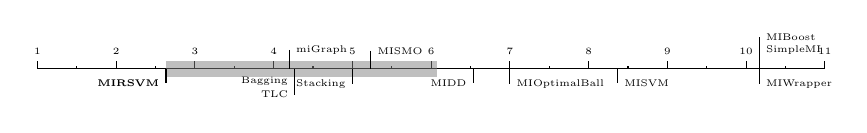
\begin{tikzpicture}
\draw (1,0) -- (11,0);
\foreach \x in {1,2,3,4,5,6,7,8,9,10,11} {
\draw (\x, 0) -- ++(0,.1) node [above,scale=0.7] {\tiny \x};
\ifthenelse{\x < 11}{\draw (\x+.5, 0) -- ++(0,.03);}{}
}

\coordinate (c0) at (2.6333,0);
\coordinate (c1) at (4.2,0);
\coordinate (c2) at (10.1667,0);
\coordinate (c3) at (7,0);
\coordinate (c4) at (6.5333,0);
\coordinate (c5) at (10.1667,0);
\coordinate (c6) at (5.2333,0);
\coordinate (c7) at (8.3667,0);
\coordinate (c8) at (10.1667,0);
\coordinate (c9) at (4.2667,0);
\coordinate (c10) at (4.2667,0);
\coordinate (c11) at (5,0);

\node (l0) at (c0) [below left=.05cm and 0cm, align=right,scale=0.7] {\tiny \textbf{MIRSVM}};
\node (l1) at (c1) [above right=.1cm and 0cm, align=left,scale=0.7] {\tiny miGraph};
\node (l2) at (c2) [above right=.27cm and 0cm, align=right,scale=0.7] {\tiny MIBoost};
\node (l3) at (c3) [below right=.05cm and 0cm, align=left,scale=0.7] {\tiny MIOptimalBall};
\node (l4) at (c4) [below left=.05cm and 0cm, align=right,scale=0.7] {\tiny MIDD};
\node (l5) at (c5) [below right=.05cm and 0cm, align=left,scale=0.7] {\tiny MIWrapper};
\node (l6) at (c6) [above right=.1cm and 0cm, align=left,scale=0.7] {\tiny MISMO};
\node (l7) at (c7) [below right=.05cm and 0cm, align=left,scale=0.7] {\tiny MISVM};
\node (l8) at (c8) [above right=.1cm and 0cm, align=left,scale=0.7] {\tiny SimpleMI};
\node (l9) at (c9) [below left=.2cm and 0cm, align=right,scale=0.7] {\tiny TLC};
\node (l10) at (c10) [below left=.02cm and 0cm, align=right,scale=0.7] {\tiny Bagging};
\node (l11) at (c11) [below left=.05cm and 0cm, align=right,scale=0.7] {\tiny Stacking};

\fill[fill=gray,fill opacity=0.5] (2.6333,-0.1) rectangle (6.0683,0.1);

\foreach \x in {0,1,2,3,4,5,6,7,8,9,10,11} {
\draw (l\x) -| (c\x);
};
\end{tikzpicture}}\vspace{-0.6em}
\captionof{figure}{Bonferroni-Dunn test for Cohen's Kappa rate}\label{fig:BonfDunnkappa}
\vspace{-0.5em}
\captionof{table}{Holm and Wilcoxon tests for Cohen's Kappa rate}\label{tab:statkappa}
\scriptsize
\resizebox{0.95\textwidth}{!}{\begin{tabular}{lccccccccccc}
\noalign{\smallskip}\hline\noalign{\smallskip}
MIRSVM vs. &miGraph &MIBoost &MIOptimalBall &MIDD &MIWrapper &MISMO &MISVM &SimpleMI &TLC &Bagging &Stacking \\
\noalign{\smallskip}\hline\noalign{\smallskip}
Holm $p$-value &0.0500 &0.0045 &0.0071 &0.0083 &0.0050 &0.0100 &0.0063 &0.0056 &0.0167 &0.0250 &0.0125 \\\noalign{\smallskip}\hline\noalign{\smallskip}
Wilcoxon $p$-value &0.0121 &0.0001 &0.0012 &0.0012 &0.0001 &0.0006 &0.0001 &0.0001 &0.1205 & 0.2077 &0.0946 \\
Wilcoxon R$^+$ &91.500 &120.00 &113.00 &113.00 &120.00 &115.00 &119.00 &120.00 &88.000 &83.000 &90.000 \\
Wilcoxon R$^-$ &13.500 &0.0000 &7.0000 &7.0000 &0.0000 &5.0000 &1.0000 &0.0000 &32.000 &37.000 &30.000 \\
\noalign{\smallskip}\hline\noalign{\smallskip}
\end{tabular}}
\end{table}
Table~\ref{tab:kappaResults} shows the Cohen's Kappa rate results obtained by the algorithms. These results support the accuracy achieved by the algorithms, in the sense that the instance-based and wrapper methods perform worse than bag-based and ensemble learners. MIRSVM's kappa values all fall within the range ($0.5$-$1$], indicating that its merit as a classifier agrees with the class distribution and is not random. Note that MIOptimalBall, MIDD, MISVM, MISMO, and Stacking contain some negative kappa values, indicating performance worse than the default-hypothesis. MIBoost, SimpleMI, and MIWrapper are shown to randomly classify all $15$ datasets. Figure~\ref{fig:BonfDunnkappa} and Table~\ref{tab:statkappa} show the results of the statistical analysis on the Cohen's Kappa Rate results. The Holm and Wilcoxon procedures reflect results similar to the Bonferroni-Dunn test, where MIRSVM performs significantly better than MIOptimalBall, MIDD, MISVM, MIWrapper, MIBoost, and SimpleMI, having $p$-values $< 0.01$. This supports MIRSVM's performance as a competitive classifier.

\subsection{AUC}
\begin{table}[b!]
\caption{AUC}\label{tab:aucResults}
\resizebox{0.95\textwidth}{!}{\begin{tabular}{lccccccccccccc}
\hline\noalign{\smallskip}
Datasets &MIRSVM & miGraph & MIBoost &MIOptimalBall &MIDD &MIWrapper &MISMO &MISVM &SimpleMI &TLC &Bagging &Stacking \\
\hline\noalign{\smallskip}
suramin &\textbf{0.8333} &\textbf{0.8333} &0.5000 &0.7250 &0.4250 &0.5000 &0.7250 &0.5000 &0.5000 &0.6000 &0.6650 &0.4524 &  \\
eastWest &\textbf{0.8000} &0.7000 &0.5000 &0.7250 &0.6125 &0.5000 &0.7125 &0.5625 &0.5000 &0.6000 &0.6000 &0.4500 &  \\
westEast &0.7500 &0.7500 &0.5000 &0.3750 &0.4500 &0.5000 &0.7375 &0.4125 &0.5000 &0.5625 &\textbf{0.8456} &0.6375 &  \\
musk1 &\textbf{0.9005} &0.8135 &0.5000 &0.7676 &0.8797 &0.5000 &0.7816 &0.7589 &0.5000 &0.8589 &0.6837 &0.8589 &  \\
musk2 &\textbf{0.8406} &0.6904 &0.5000 &0.7432 &0.6981 &0.5000 &0.6772 &0.6900 &0.5000 &0.6317 &0.6732 &0.6435 &  \\
webmining &0.6320 &0.5000 &0.5000 &0.5096 &0.5000 &0.5000 &0.7184 &0.8098 &0.5000 &0.6837 &\textbf{0.8123} &0.6048 &  \\
trx &0.6500 &0.6170 &0.5000 &\textbf{0.7392} &0.6932 &0.5000 &0.5000 &0.5000 &0.5000 &0.6732 &0.6450 &0.6281 &  \\
mutagenesis-atoms &0.7106 &0.7137 &0.5000 &0.5824 &0.6186 &0.5000 &0.6420 &0.5000 &0.5000 &\textbf{0.7257} &\textbf{0.7257} &0.7137 &  \\
mutagenesis-bonds &0.7856 &0.7455 &0.5000 &0.6578 &0.6981 &0.5000 &0.7850 &0.5000 &0.5000 &0.8012 &0.8012 &\textbf{0.8211} &  \\
mutagenesis-chains &\textbf{0.8252} &0.7417 &0.5000 &0.6142 &0.7257 &0.5000 &0.8051 &0.5000 &0.5000 &0.8170 &0.8170 &0.8130 &  \\
tiger &0.7750 &0.7950 &0.5000 &0.5000 &0.7100 &0.5000 &0.7200 &0.7550 &0.5000 &0.6650 &\textbf{0.8000} &0.7250 &  \\
elephant &0.8200 &\textbf{0.8300} &0.5000 &0.5000 &0.7900 &0.5000 &0.8100 &0.8000 &0.5000 &0.8000 &0.5625 &0.8250 &  \\
fox &0.6550 &0.6300 &0.5000 &0.5000 &0.5800 &0.5000 &0.5250 &0.4750 &0.5000 &0.6450 &\textbf{0.8589} &0.6500 &  \\
component &0.7855 &0.7496 &0.5000 &0.5536 &0.6033 &0.5000 &0.6272 &0.5201 &0.5000 &\textbf{0.8123} &0.6000 &0.8081 &  \\
function &0.7563 &0.7698 &0.5000 &0.5298 &0.6015 &0.5000 &0.6391 &0.5268 &0.5000 &\textbf{0.8456} &0.6317 &0.8434 &  \\
\noalign{\smallskip}\hline\noalign{\smallskip}
Average &\textbf{0.7680} &0.7253 &0.5000 &0.6015 &0.6390 &0.5000 &0.6937 &0.5874 &0.5000 &0.7148 &0.7148 &0.6983 &  \\
Rank &\textbf{2.7667} &4.2667 &10.1667 &7.0000 &6.5333 &10.1667 &5.2333 &8.2333 &10.1667 &4.2667 &4.2667 &4.9333 &  \\
\hline\noalign{\smallskip}
\end{tabular}}
\centering
\resizebox{0.95\textwidth}{!}{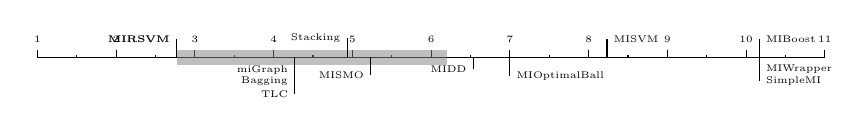
\begin{tikzpicture}
\draw (1,0) -- (11,0);
\foreach \x in {1,2,3,4,5,6,7,8,9,10,11} {
\draw (\x, 0) -- ++(0,.1) node [above,scale=0.7] {\tiny \x};
\ifthenelse{\x < 11}{\draw (\x+.5, 0) -- ++(0,.03);}{}
}

\coordinate (c0) at (2.7667,0);
\coordinate (c1) at (4.2667,0);
\coordinate (c2) at (10.1667,0);
\coordinate (c3) at (7,0);
\coordinate (c4) at (6.5333,0);
\coordinate (c5) at (10.1667,0);
\coordinate (c6) at (5.2333,0);
\coordinate (c7) at (8.2333,0);
\coordinate (c8) at (10.1667,0);
\coordinate (c9) at (4.2667,0);
\coordinate (c10) at (4.2667,0);
\coordinate (c11) at (4.9333,0);

\node (l0) at (c0) [above left=.1cm and 0cm, align=right,scale=0.7] {\tiny \textbf{MIRSVM}};
\node (l1) at (c1) [below left=.02cm and 0cm, align=right,scale=0.7] {\tiny miGraph};
\node (l2) at (c2) [above right=.1cm and 0cm, align=left,scale=0.7] {\tiny MIBoost};
\node (l3) at (c3) [below right=.1cm and 0cm, align=left,scale=0.7] {\tiny MIOptimalBall};
\node (l4) at (c4) [below left=.02cm and 0cm, align=right,scale=0.7] {\tiny MIDD};
\node (l5) at (c5) [below right=.01cm and 0cm, align=left,scale=0.7] {\tiny MIWrapper};
\node (l6) at (c6) [below left=.1cm and 0cm, align=right,scale=0.7] {\tiny MISMO};
\node (l7) at (c7) [above right=.1cm and 0cm, align=left,scale=0.7] {\tiny MISVM};
\node (l8) at (c8) [below right=.16cm and 0cm, align=left,scale=0.7] {\tiny SimpleMI};
\node (l9) at (c9) [below left=.34cm and 0cm, align=right,scale=0.7] {\tiny TLC};
\node (l10) at (c10) [below left=.16cm and 0cm, align=right,scale=0.7] {\tiny Bagging};
\node (l11) at (c11) [above left=.1cm and 0cm, align=right,scale=0.7] {\tiny Stacking};

\fill[fill=gray,fill opacity=0.5] (2.7667,-0.1) rectangle (6.2017,0.1);

\foreach \x in {0,1,2,3,4,5,6,7,8,9,10,11} {
\draw (l\x) -| (c\x);
};
\end{tikzpicture}}\vspace{-0.6em}
\captionof{figure}{Bonferroni-Dunn test for AUC}\label{fig:BonfDunnauc}
\vspace{-0.5em}
\captionof{table}{Holm and Wilcoxon tests for AUC}\label{tab:statauc}
\scriptsize
\resizebox{0.95\textwidth}{!}{\begin{tabular}{lccccccccccc}
\noalign{\smallskip}\hline\noalign{\smallskip}
MIRSVM vs. &miGraph &MIBoost &MIOptimalBall &MIDD &MIWrapper &MISMO &MISVM &SimpleMI &TLC &Bagging &Stacking \\
\noalign{\smallskip}\hline\noalign{\smallskip}
Holm $p$-value &0.0167 &0.0045 &0.0071 &0.0083 &0.0050 &0.0100 &0.0063 &0.0056 &0.0250 &0.0500 &0.0125 \\\noalign{\smallskip}\hline\noalign{\smallskip}
Wilcoxon $p$-value &0.0166 &0.0001 &0.0002 &0.0003 &0.0001 &0.0012 &0.0009 &0.0001 & 0.2523 & 0.3028 &0.0781 \\
Wilcoxon R$^+$ &90.000 &120.00 &118.00 &117.00 &120.00 &113.00 &114.00 &120.00 &81.000 &79.000 &91.500 \\
Wilcoxon R$^-$ &15.000 &0.0000 &2.0000 &3.0000 &0.0000 &7.0000 &6.0000 &0.0000 &39.000 &41.000 &28.500 \\
\noalign{\smallskip}\hline\noalign{\smallskip}
\end{tabular}}
\end{table}
Table~\ref{tab:aucResults} shows AUC results obtained by the algorithms, which complement the accuracy and kappa rate, emphasizing the better performance of bag-based methods. MIRSVM achieves the best AUC score on $5$ of the $15$ datasets, while MIBoost, SimpleMI, and MIWrapper obtain the worst results. Their AUC score indicates random predictor behavior, having values $= 0.5$. Bag-level methods all obtain scores between $0.7$ and $0.77$ indicating a high true positive rate and a low false positive rate, which is reflected by the precision and recall results. Figure~\ref{fig:BonfDunnauc} and Table~\ref{tab:statauc} show that MIRSVM performs significantly better than $6$ out of the $11$ competing algorithms. Holm's procedure indicates that significant differences exist between MIRSVM and all algorithms except miGraph, TLC, Bagging, and Stacking. MISVM's true positive rate could be affected because of the possible imbalance of support vectors from the positive and negative classes (favoring the negative). Note that the Wilcoxon $p$-values for MIWrapper, MIBoost, and SimpleMI are $0.0001$. 

\subsection{Overall Comparison}
\begin{table}[t!]
\centering
\caption{Run Time (seconds)}\label{tab:time}
\resizebox{0.95\textwidth}{!}{\begin{tabular}{lrrrrrrrrrrrrr}
\hline\noalign{\smallskip}
Datasets &MIRSVM & miGraph & MIBoost &MIOptimalBall &MIDD &MIWrapper &MISMO &MISVM &SimpleMI &TLC &Bagging &Stacking \\
\hline\noalign{\smallskip}
suramin &\textbf{0.1} &19.7 &8.8 &30.5 &7922.0 &9.5 &52.3 &333.9 &7.2 &35.5 &183.0 &90.6 &  \\
eastWest &\textbf{0.1} &3.0 &5.5 &9.4 &217.1 &6.3 &14.8 &21.4 &5.8 &15.4 &15.4 &15.2 &  \\
westEast &\textbf{0.1} &2.8 &6.5 &7.8 &79.7 &6.5 &14.7 &99.5 &6.0 &16.6 &12128.1 &10.8 &  \\
musk1 &\textbf{0.4} &56.8 &13.4 &32.1 &3542.6 &20.6 &89.7 &198.4 &11.1 &93.0 &86272.6 &759.5 &  \\
musk2 &\textbf{2.3} &452.3 &97.3 &782.9 &126016.8 &208.3 &1799.4 &26093.5 &16.1 &1772.2 &2229.3 &16759.0 &  \\
webmining &\textbf{300.6} &302.5 &45745.4 &60474.8 &47601.4 &68736.7 &51923.6 &105622.3 &2685.9 &86272.6 &9861.5 &592948.9 &  \\
trx &61.8 &2206.4 &17.6 &682.3 &339110.5 &19.3 &8670.3 &134622.1 &\textbf{7.4} &2229.3 &243.3 &11927.9 &  \\
mutagenesis-atoms &9.8 &193.1 &8.8 &99.2 &2623.0 &8.0 &55.0 &53.5 &\textbf{6.4} &44.0 &44.0 &153.9 &  \\
mutagenesis-bonds &\textbf{8.3} &410.3 &10.2 &310.2 &17538.7 &12.3 &457.4 &2794.8 &8.4 &131.1 &131.1 &853.1 &  \\
mutagenesis-chains &19.3 &513.4 &12.0 &525.0 &48982.7 &14.8 &2451.9 &6637.4 &\textbf{7.2} &224.4 &224.4 &1619.0 &  \\
tiger &29.5 &302.8 &44.5 &157.8 &23220.5 &56.2 &208.0 &608.8 &\textbf{16.2} &183.0 &212.1 &1085.0 &  \\
elephant &47.7 &306.7 &45.5 &243.9 &56456.2 &69.7 &232.1 &1114.3 &20.8 &212.1 &\textbf{16.6} &1462.2 &  \\
fox &81.0 &303.1 &44.2 &206.1 &27773.8 &66.0 &369.6 &891.5 &\textbf{23.5} &243.3 &93.0 &1729.1 &  \\
component &231.7 &3091.0 &572.5 &228209.6 &96263.9 &1096.9 &629366.4 &37224.6 &144.0 &9861.5 &\textbf{35.5} &79149.8 &  \\
function &740.3 &8162.7 &935.5 &768458.0 &350124.7 &1887.5 &1052225.3 &565026.4 &\textbf{232.8} &12128.1 &1772.2 &185918.5 &  \\
\noalign{\smallskip}\hline\noalign{\smallskip}
Average &\textbf{102.2} &1088.4 &3171.2 &70682.0 &76498.2 &4814.6 &116528.7 &58756.2 &213.3 &7564.1 &7564.1 &59632.2 &  \\
Rank &2.3 &6.2 &3.1 &7.2 &11.1 &4.3 &8.5 &10.1 &\textbf{1.9} &7.2 &6.5 &9.7 &  \\
\hline\noalign{\smallskip}
\end{tabular}}
\captionof{table}{Overall ranks comparison}\label{tab:metarank}
\resizebox{0.95\textwidth}{!}{\begin{tabular}{lccccccccccccc}
\hline\noalign{\smallskip}
Ranks &MIRSVM & miGraph & MIBoost &MIOptimalBall &MIDD &MIWrapper &MISMO &MISVM &SimpleMI &TLC &Bagging &Stacking \\
\midrule
Accuracy &\textbf{2.2000} &3.8667 &9.6000 &7.8667 &6.5667 &9.6000 &5.3333 &8.5667 &9.6000 &4.7000 &4.8667 &5.2333 &  \\
Precision &\textbf{5.3333} &6.1333 &7.1000 &7.3333 &7.3667 &7.1000 &5.8667 &5.8667 &7.1000 &5.9000 &6.3333 &6.5667 &  \\
Recall &4.8667 &6.5667 &6.8667 &6.3333 &7.3667 &6.8667 &6.7000 &7.4333 &\textbf{4.8333} &7.3667 &6.0667 &6.7333 &  \\
Kappa &\textbf{2.6333} &4.2000 &10.1667 &7.0000 &6.5333 &10.1667 &5.2333 &8.3667 &10.1667 &4.2667 &4.2667 &5.0000 &  \\
AUC &\textbf{2.7667} &4.2667 &10.1667 &7.0000 &6.5333 &10.1667 &5.2333 &8.2333 &10.1667 &4.2667 &4.2667 &4.9333 &  \\
Time &2.2667 &6.2000 &3.1000 &7.2000 &11.0667 &4.3000 &8.5333 &10.1333 &\textbf{1.8667} &7.2000 &6.4667 &9.6667 &  \\
\noalign{\smallskip}\hline\noalign{\smallskip}
Average &\textbf{3.3444} &5.2056 &7.8333 &7.1222 &7.5722 &8.0333 &6.1500 &8.1000 &7.2889 &5.6167 &5.3778 &6.3556 &  \\
Rank &\textbf{1.3333} &3.6667 &8.9167 &7.7500 &9.2500 &9.0833 &5.9167 &8.7500 &7.3333 &5.2500 &4.2500 &6.5000 &  \\
\hline\noalign{\smallskip}
\end{tabular}}
\centering
\resizebox{0.95\textwidth}{!}{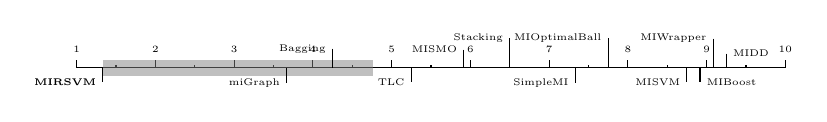
\begin{tikzpicture}
\draw (1,0) -- (10,0);
\foreach \x in {1,2,3,4,5,6,7,8,9,10} {
\draw (\x, 0) -- ++(0,.1) node [above,scale=0.7] {\tiny \x};
\ifthenelse{\x < 10}{\draw (\x+.5, 0) -- ++(0,.03);}{}
}

\coordinate (c0) at (1.3333,0);
\coordinate (c1) at (3.6667,0);
\coordinate (c2) at (8.9167,0);
\coordinate (c3) at (7.75,0);
\coordinate (c4) at (9.25,0);
\coordinate (c5) at (9.0833,0);
\coordinate (c6) at (5.9167,0);
\coordinate (c7) at (8.75,0);
\coordinate (c8) at (7.3333,0);
\coordinate (c9) at (5.25,0);
\coordinate (c10) at (4.25,0);
\coordinate (c11) at (6.5,0);

\node (l0) at (c0) [below left=.05cm and 0cm, align=right,scale=0.7] {\tiny \textbf{MIRSVM}};
\node (l1) at (c1) [below left=.05cm and 0cm, align=right,scale=0.7] {\tiny miGraph};
\node (l2) at (c2) [below right=.05cm and 0cm, align=left,scale=0.7] {\tiny MIBoost};
\node (l3) at (c3) [above left=.23cm and 0cm, align=right,scale=0.7] {\tiny MIOptimalBall};
\node (l4) at (c4) [above right=.05cmand 0cm, align=left,scale=0.7] {\tiny MIDD};
\node (l5) at (c5) [above left=.23cm and 0cm, align=right,scale=0.7] {\tiny MIWrapper};
\node (l6) at (c6) [above left=.1cm and 0cm, align=right,scale=0.7] {\tiny MISMO};
\node (l7) at (c7) [below left=.05cm and 0cm, align=right,scale=0.7] {\tiny MISVM};
\node (l8) at (c8) [below left=.05cm and 0cm, align=right,scale=0.7] {\tiny SimpleMI};
\node (l9) at (c9) [below left=.05cm and 0cm, align=right,scale=0.7] {\tiny TLC};
\node (l10) at (c10) [above left=.1cm and 0cm, align=right,scale=0.7] {\tiny Bagging};
\node (l11) at (c11) [above left=.23cm and 0cm, align=right,scale=0.7] {\tiny Stacking};

\fill[fill=gray,fill opacity=0.5] (1.3333,-0.1) rectangle (4.7683,0.1);

\foreach \x in {0,1,2,3,4,5,6,7,8,9,10,11} {
\draw (l\x) -| (c\x);
};
\end{tikzpicture}}\vspace{-0.6em}
\captionof{figure}{Bonferroni-Dunn test for overall ranks comparison}\label{fig:BonfDunnpmeta}
\end{table}
Table~\ref{tab:time} shows the run times, in seconds, for each algorithm. MIRSVM has the fastest run time and is ranked second. MIRSVM shows very good scalability considering the number of features, such as in the webmining dataset which comprises of $5863$ attributes. Additionally, taking into account the number of instances as seen in the two largest datasets, component and function, MIRSVM displays superior scalability. It is important to note that quadratic programming solvers are not the most efficient tools for solving optimization problems in terms of run time, and yet MIRSVM still is shown to perform competitively against the current state-of-the-art algorithms. The scalability of MIRSVM is founded on the speedy rate of bag-representative convergence, as shown previously in Figure~\ref{fig:convegence}.

SimpleMI achieves the highest rank and competitive run times because, rather than use the instances in each bag to train a model, it takes the mean value of the instances in a bag and uses that for training. Even though SimpleMI has fast run-times, its performance over the previous metrics has been shown to be random and not as effective as the bag-level methods.

Table~\ref{tab:metarank} shows the ranks achieved by each of the metrics along with the average and meta-ranks, to illustrate the overall performance across all metrics. MIRSVM has the best meta-rank (rank of the ranks) and the miGraph method has the second best. The meta-ranks also highlight the better performance of bag-level methods over instance-level and wrapper methods, emphasizing the importance of training at the bag-level. Not only does MIRSVM use bag-level information during classification, but it also optimizes over the instances within the bag, which helps determine which instances contribute the most information about the bags label. SimpleMI, MIWrapper, MIBoost, MISVM, and MDD have the worst performance compared to MIRSVM and miGraph. Specifically, it is evident from the precision and recall results that MIBoost, MIWrapper, and SimpleMI, for example, classify all bags as negative for datasets that have imbalanced class distributions which favor the negative class. This emphasizes the disadvantage of using wrapper methods and assuming the data distribution of the instances within positive bags. Although these algorithms are popular in literature, the experimental study clearly shows that recent bag-level and ensemble methods easily overcome traditional multi-instance learning algorithms. 

In summary, MIRSVM offers improvement in terms of both accuracy and run-time when compared to referenced methods, especially those utilizing SVM-based algorithms.

\section{Conclusion}\label{sec:conclusion}
This paper proposed a novel formulation and algorithm for the multiple-instance support vector machine problem, which optimizes bag classification via bag-representative selection. First, the primal formulation was posed and its dual was then derived and solution computed using a quadratic programming solver. This formulation was designed to utilize bag-level information and find an optimal separating hyperplane between bags, rather than individual instances, using the standard multi-instance assumption. The SMI assumption states that a bag is labeled positive if and only if at least one instance within a bag is positive, and is negative otherwise. The key features of the proposed algorithm MIRSVM are its ability to identify instances within positive and negative bags, i.e. the support vectors or representatives, that highly impact the decision boundary and margin, as well as avoiding uncertainties and issues caused by techniques that flatten, subset, or under-represent positive instances within positively labeled bags. Additionally, it exhibits desirable convergence and scalability, making it suitable for large-scale learning tasks.

The experimental study showed the better performance of MIRSVM compared with state-of-the-art multi-instance support vector machines, traditional multi-instance learners, as well as ensemble methods. The results, according to a variety of performance metrics, were compared and further validated using statistical analysis with non-parametric tests which highlight the advantages of using bag-level based and ensemble learners, such as miGraph, Bagging, and Stacking, while showing the instance-level based learners performed poorly in comparison or were deemed as strongly biased and unstable classifiers. Our proposal, MIRSVM, performs statistically better, neither compromising accuracy nor run-time while displaying a robust performance across all of the evaluated datasets.

\section*{Acknowledgment}
This research was supported by the Spanish Ministry of Economy and Competitiveness, project TIN2014-55252-P, and by FEDER funds.

% BibTeX users please use one of
\bibliographystyle{elsarticle-num-names}
\bibliography{references}   

\end{document}


